\documentclass[final]{beamer}
\def\PosterFull{1}
% Fixed outer geometry for the IAS 2026 poster and its standalone previews.
% Edit this file only when changing the composition of the whole poster.
\def\PosterLayoutLoaded{1}
\newcommand{\PosterOuterMargin}{23mm}
\newcommand{\PosterColumnGap}{8mm}
\newcommand{\PosterRowGap}{4mm}
\newcommand{\PosterGridWidthMm}{868.4}
\newcommand{\PosterGridWidth}{\PosterGridWidthMm mm}
\newcommand{\PosterIdentityLeft}{8mm}
\newcommand{\PosterIdentityWidthMm}{898.4}
\newcommand{\PosterIdentityWidth}{\PosterIdentityWidthMm mm}
\newcommand{\PosterIdentityHeightMm}{54}
\newcommand{\PosterGreenHeightMm}{86}
\newcommand{\PosterHeaderHeightMm}{140}
\newcommand{\PosterHeaderHeight}{\PosterHeaderHeightMm mm}
\newcommand{\PosterGreenInset}{15mm}
\newcommand{\PosterHeaderTopOffset}{-3mm}
\newcommand{\PosterPhysicalPageWidthCm}{91.44}
\newcommand{\PosterPhysicalPageHeightCm}{106.68}

\newcommand{\PosterColWidth}{284.13mm}

\newcommand{\PosterRowHeight}{258mm}
\newcommand{\PosterRowHeightC}{352mm}
\newcommand{\PosterRowHeightA}{200mm}
% Module envelopes: width x height. Interior drawings remain local to each file.
\newcommand{\PosterOneWidth}{224mm}
\newcommand{\PosterTwoWidth}{412.4mm}
\newcommand{\PosterThreeWidth}{216mm}
\newcommand{\PosterTopRowHeight}{200mm}
\newcommand{\PosterStripHeight}{44mm}
\newcommand{\PosterFourHeight}{140mm}
\newcommand{\PosterHalfWidth}{430.2mm}
\newcommand{\PosterMiddleRowHeight}{140mm}
\newcommand{\PosterLowerRowHeight}{160mm}
\newcommand{\PosterBottomRowHeightMm}{84}
\newcommand{\PosterBottomRowHeight}{\PosterBottomRowHeightMm mm}

% Preview page sizes are centimetre numbers consumed by beamerposter.
\newcommand{\PosterPreviewTop}{6mm}
\newcommand{\PosterPreviewFullPageWidth}{\PosterPhysicalPageWidthCm}
\newcommand{\PosterPreviewWhitePageHeight}{8.0}
\newcommand{\PosterPreviewGreenPageHeight}{11.2}
\newcommand{\PosterPreviewTopRowPageHeight}{22.6}
\newcommand{\PosterPreviewStripPageHeight}{7.0}
\newcommand{\PosterPreviewFourPageHeight}{16.6}
\newcommand{\PosterPreviewMiddlePageHeight}{16.4}
\newcommand{\PosterPreviewLowerPageHeight}{18.6}
\newcommand{\PosterPreviewBottomPageHeight}{11.0}
\newcommand{\PosterPreviewOnePageWidth}{24.8}
\newcommand{\PosterPreviewTwoPageWidth}{43.6}
\newcommand{\PosterPreviewThreePageWidth}{23.84}
\newcommand{\PosterPreviewHalfPageWidth}{46.2}
\newcommand{\PosterPreviewOneLeft}{12mm}
\newcommand{\PosterPreviewTwoLeft}{11.8mm}
\newcommand{\PosterPreviewThreeLeft}{11.2mm}
\newcommand{\PosterPreviewHalfLeft}{15.9mm}

\def\PosterPageWidth{\PosterPhysicalPageWidthCm}
\def\PosterPageHeight{\PosterPhysicalPageHeightCm}
\usepackage[size=custom,width=\PosterPageWidth,height=\PosterPageHeight,scale=1.0]{beamerposter}
\usepackage{fontspec}
\usepackage{unicode-math}
\usepackage{amsmath,amssymb,mathtools}
\usepackage{graphicx}
\usepackage{tikz}
\usetikzlibrary{calc,positioning,shapes.geometric,shapes.misc,arrows.meta,patterns}
\usepackage{pgfplots}
\pgfplotsset{compat=1.18}
\usepackage{booktabs,tabularx,array}
\usepackage{ragged2e}
\usepackage[most]{tcolorbox}
\tcbuselibrary{skins,breakable}

% Shared visual roles and components, then scientific values used by the sections.
% IAS 2026 poster design system: palette, typography, spacing, and components.
% The paired DESIGN_SYSTEM.md documents each token and its intended use.
% Palette sampled from the approved poster reference, with accessible plot markers.
\definecolor{IASDarkGreen}{HTML}{003B2D}
\definecolor{IASDeepGreen}{HTML}{00291F}
\definecolor{IASHeaderGreen}{HTML}{004A3A}
\definecolor{IASMidGreen}{HTML}{00664B}
\definecolor{IASGold}{HTML}{C99A20}
\definecolor{IASWhite}{HTML}{FFFFFF}
% Legacy figure code uses this name for node fills; keep it neutral white.
\colorlet{IASIvory}{IASWhite}
\definecolor{IASDarkText}{HTML}{17372D}
\definecolor{IASPaleGreen}{HTML}{EAF2ED}
\definecolor{IASPaleGold}{HTML}{FFF4D6}
\definecolor{IASBlue}{HTML}{176494}
\definecolor{IASVermillion}{HTML}{BC3030}
\definecolor{IASGray}{HTML}{5F6B66}
\definecolor{IASRule}{HTML}{CFDDD5}
\usetheme{IAS2026}

\setmainfont{TeX Gyre Heros}[Ligatures=TeX]
\setsansfont{TeX Gyre Heros}[Ligatures=TeX]
\setmathfont{Latin Modern Math}
\newfontfamily\PosterCondensed{TeX Gyre Heros Cn}[Ligatures=TeX]
\setbeamertemplate{background canvas}{\color{IASWhite}\rule{\paperwidth}{\paperheight}}
\setbeamertemplate{navigation symbols}{}
\setbeamersize{text margin left=0mm,text margin right=0mm}
\setlength{\parindent}{0pt}
\setlength{\parskip}{0pt}
\setlength{\textwidth}{\paperwidth}
\setlength{\textheight}{\paperheight}
\pagestyle{empty}
\pagecolor{IASWhite}

\newcommand{\PosterPending}{\textcolor{IASGray}{\bfseries PENDING}}
\newcommand{\StableMark}{\tikz[baseline=-0.65ex]\node[circle,fill=IASBlue,draw=IASBlue,inner sep=2.1pt] {};}
\newcommand{\UnstableMark}{\tikz[baseline=-0.55ex]\node[cross out,draw=IASVermillion,line width=1.5pt,minimum size=5.2mm,inner sep=0pt] {};}
\newcommand{\BoundaryMark}{\tikz[baseline=-0.55ex]\node[diamond,fill=IASGold,draw=IASGold,minimum size=5.0mm,inner sep=0pt] {};}
\newcommand{\UnresolvedMark}{\tikz[baseline=-0.55ex]\node[circle,draw=IASGray,line width=1.3pt,minimum size=4.8mm,inner sep=0pt] {};}
\newcommand{\HasseFullMark}{\tikz[baseline=-0.55ex]\node[circle,draw=IASVermillion,fill=IASVermillion,minimum size=5mm,inner sep=0pt] {};}
\newcommand{\CandidateBusMark}{\tikz[baseline=-0.55ex]\node[circle,draw=IASVermillion,fill=IASVermillion,minimum size=5mm,inner sep=0pt] {};}
\newcommand{\PosterBody}{\fontsize{34.2pt}{39pt}\selectfont}
\newcommand{\PosterParagraph}{\PosterBody\color{IASDarkText}\raggedright}
\newcommand{\Subhead}{\PosterCondensed\bfseries\fontsize{38pt}{41pt}\selectfont}
\newcommand{\PosterMathSpacing}{%
  \setlength{\abovedisplayskip}{3mm}\setlength{\belowdisplayskip}{3mm}%
  \setlength{\abovedisplayshortskip}{2mm}\setlength{\belowdisplayshortskip}{2mm}}
\newcommand{\EquationSize}{\fontsize{36pt}{41pt}\selectfont\PosterMathSpacing}
\newcommand{\HeroEquation}{\fontsize{44pt}{48pt}\selectfont\PosterMathSpacing}
\newcommand{\MetricSize}{\fontsize{38pt}{42pt}\selectfont}
\newcommand{\TableSize}{\fontsize{26pt}{29pt}\selectfont}
\newcommand{\FigureSize}{\fontsize{24.7pt}{27.2pt}\selectfont}
% Semantic type roles; keep the names stable when retuning the type scale.
\newcommand{\PosterHeaderEyebrow}{\bfseries\fontsize{25pt}{28pt}\selectfont}
\newcommand{\PosterHeroTitle}{\PosterCondensed\bfseries\fontsize{90pt}{94pt}\selectfont}
\newcommand{\PosterHeaderSubtitle}{\bfseries\fontsize{36pt}{40pt}\selectfont}
\newcommand{\PosterHeaderByline}{\bfseries\fontsize{30pt}{34pt}\selectfont}
\newcommand{\PosterPanelBadgeType}{\PosterCondensed\bfseries\fontsize{36pt}{36pt}\selectfont}
\newcommand{\PosterPanelHeadingType}{\PosterCondensed\bfseries\fontsize{43pt}{46pt}\selectfont}
\newcommand{\PosterTicketHeadingType}{\PosterCondensed\bfseries\fontsize{44pt}{47pt}\selectfont}
\newcommand{\PosterMetricValueType}{\PosterCondensed\bfseries\fontsize{40pt}{42pt}\selectfont}
\newcommand{\PosterMetricLabelType}{\bfseries\fontsize{27pt}{30pt}\selectfont}
\newcommand{\PosterMetricDetailType}{\fontsize{24.2pt}{26.2pt}\selectfont}
\newcommand{\PosterFooterKickerType}{\PosterCondensed\bfseries\fontsize{24pt}{27pt}\selectfont}
\newcommand{\PosterFooterTitleType}{\PosterCondensed\bfseries\fontsize{56pt}{59pt}\selectfont}
\newcommand{\PosterFooterSummaryType}{\fontsize{29pt}{32pt}\selectfont}
\newcommand{\PosterFooterReferenceType}{\fontsize{19pt}{22pt}\selectfont}
\newcommand{\PosterFooterReferenceHeadingType}{\PosterCondensed\bfseries\fontsize{23pt}{26pt}\selectfont}
\newcommand{\PosterFooterContactHeadingType}{\PosterCondensed\bfseries\fontsize{25pt}{28pt}\selectfont}
\newcommand{\PosterFooterContactNameType}{\bfseries\fontsize{23pt}{26pt}\selectfont}
\newcommand{\PosterFooterContactLineType}{\fontsize{21pt}{24pt}\selectfont}
\newcommand{\PosterFooterQrLabelType}{\PosterCondensed\bfseries\fontsize{19pt}{21pt}\selectfont}

% Interior spacing and panel anatomy. Outer grid values live in poster_layout.tex.
\newcommand{\PosterPanelTitleHeight}{32mm}
\newcommand{\PosterTicketTitleHeight}{36mm}
\newcommand{\PosterPanelBadgeWidth}{21mm}
\newcommand{\PosterPanelBadgeDiameter}{17.5mm}
\newcommand{\PosterPanelTitleInset}{2mm}
\newcommand{\PosterPanelTitleGap}{2.5mm}
\newcommand{\PosterPanelContentInset}{26mm}
\newcommand{\PosterPanelBorder}{1.1pt}
\newcommand{\PosterPanelCornerRadius}{3mm}
\newcommand{\PosterPanelPaddingX}{3mm}
\newcommand{\PosterPanelPaddingTop}{4mm}
\newcommand{\PosterPanelPaddingBottom}{2mm}
\newcommand{\PosterMetricCellHeight}{40mm}
\newcommand{\PosterIASLogoWidth}{137mm}
\newcommand{\PosterUniandesLogoWidth}{120mm}
\newcommand{\StatusPending}[1]{{\bfseries\color{IASGray}#1}}
\newcommand{\StatusConditional}[1]{{\bfseries\color{IASGold!70!black}#1}}
\newcommand{\StatusPass}[1]{{\bfseries\color{IASBlue}#1}}
\newcommand{\PolicySwatch}[2]{\tikz[baseline=-0.65ex]\filldraw[fill=#1,draw=IASRule,line width=0.5pt] (0,0) rectangle (4mm,4mm);\,#2}

\newcommand{\PosterBadge}[1]{\tikz[baseline={([yshift=-5.5mm]n.center)}]\node[circle,fill=IASGold,draw=IASWhite,line width=1.3pt,text=IASDarkGreen,minimum size=\PosterPanelBadgeDiameter,inner sep=0pt,text height=8.4mm,text depth=0pt,font=\PosterPanelBadgeType](n){#1};}

\newcommand{\PosterPanelTitle}[2]{%
  \begin{minipage}[c][\PosterPanelTitleHeight][c]{\linewidth}\hspace{\PosterPanelTitleInset}%
    \begin{minipage}[c][\PosterPanelTitleHeight][c]{\PosterPanelBadgeWidth}\centering
      \PosterBadge{#1}
    \end{minipage}\hspace{\PosterPanelTitleGap}%
    \begin{minipage}[c][\PosterPanelTitleHeight][c]{\dimexpr\linewidth-\PosterPanelContentInset\relax}\raggedright
      {\PosterPanelHeadingType\color{white}#2\par}
    \end{minipage}%
  \end{minipage}%
}
\newtcolorbox{PosterPanel}[3]{
  enhanced, width=\linewidth, height=#1,
  colback=IASWhite, colframe=IASRule, colbacktitle=IASMidGreen,
  coltitle=white, boxrule=\PosterPanelBorder, arc=\PosterPanelCornerRadius,
  left=\PosterPanelPaddingX,right=\PosterPanelPaddingX,top=\PosterPanelPaddingTop,bottom=\PosterPanelPaddingBottom,boxsep=0mm,
  toptitle=0mm,bottomtitle=0mm,lefttitle=0mm,righttitle=0mm,titlerule=1.6pt,titlerule style={color=IASGold},
  title={\PosterPanelTitle{#2}{#3}},
  before skip=0pt,after skip=0pt,
  before upper={\setlength{\parskip}{0pt}\setlength{\parindent}{0pt}},
  halign title=left,
}

% Ticket 2 uses a compact local panel title; later poster bands keep PosterPanel.
\newcommand{\TicketTwoPanelTitle}[2]{%
  \begin{minipage}[c][\PosterTicketTitleHeight][c]{\linewidth}\hspace{\PosterPanelTitleInset}%
    \begin{minipage}[c][\PosterTicketTitleHeight][c]{\PosterPanelBadgeWidth}\centering
      \PosterBadge{#1}
    \end{minipage}\hspace{\PosterPanelTitleGap}%
    \begin{minipage}[c][\PosterTicketTitleHeight][c]{\dimexpr\linewidth-\PosterPanelContentInset\relax}\raggedright
      {\PosterTicketHeadingType\color{white}#2\par}
    \end{minipage}%
  \end{minipage}%
}
\newtcolorbox{TicketTwoPanel}[3]{
  enhanced, width=\linewidth, height=#1,
  colback=IASWhite, colframe=IASRule, colbacktitle=IASMidGreen,
  coltitle=white, boxrule=\PosterPanelBorder, arc=\PosterPanelCornerRadius,
  left=\PosterPanelPaddingX,right=\PosterPanelPaddingX,top=\PosterPanelPaddingTop,bottom=\PosterPanelPaddingBottom,boxsep=0mm,
  toptitle=0mm,bottomtitle=0mm,lefttitle=0mm,righttitle=0mm,titlerule=1.6pt,titlerule style={color=IASGold},
  title={\TicketTwoPanelTitle{#2}{#3}},
  before skip=0pt,after skip=0pt,
  before upper={\setlength{\parskip}{0pt}\setlength{\parindent}{0pt}},
  halign title=left,
}

% Plain-language call-out: every equation block is followed by what it means in words.
\newtcolorbox{InWords}{enhanced, colback=IASPaleGold, colframe=IASPaleGold, boxrule=0pt, arc=1.5mm,
  borderline west={1.8mm}{0pt}{IASGold}, left=4.5mm, right=3mm, top=1.8mm, bottom=1.8mm,
  before skip=0pt, after skip=0pt, fontupper=\FigureSize\color{IASDarkText}\raggedright,
  before upper={\setlength{\parskip}{0pt}\setlength{\parindent}{0pt}}}
\newcommand{\InWordsLabel}{\textbf{\color{IASGold!65!black}IN WORDS\ \ }}
\newcommand{\StepBadge}[1]{\tikz[baseline={([yshift=-2.2mm]n.center)}]\node[circle,fill=IASGold,text=IASDarkGreen,minimum size=11.5mm,inner sep=0pt,text height=3.6mm,text depth=0pt,font=\PosterCondensed\bfseries\fontsize{27pt}{27pt}\selectfont](n){#1};}

\newcommand{\MetricCell}[3]{%
  \begin{minipage}[c][\PosterMetricCellHeight][c]{\linewidth}\centering
    {\PosterMetricValueType\color{IASGold}#1\par}
    {\PosterMetricLabelType\color{white}#2\par}
    {\PosterMetricDetailType\color{IASPaleGreen}#3\par}
  \end{minipage}%
}

% Values generated from hashed evidence. Do not edit by hand.
\newcommand{\GFLPercent}{87.6}
\newcommand{\GFLMW}{4,732.82}
\newcommand{\SGMW}{669.94}
\newcommand{\AddedMW}{5.403}
\newcommand{\FreqMax}{0.4746}
\newcommand{\RocofMax}{0.2008}
\newcommand{\VoltageMin}{0.972}
\newcommand{\VoltageMax}{1.079}
\newcommand{\SlackMin}{0.00634}
\newcommand{\PanelCount}{485}
\newcommand{\RankChecks}{60}
\newcommand{\RankError}{4.85e-08}
\newcommand{\WalkMin}{18}
\newcommand{\WalkMax}{46}
\newcommand{\TargetFreq}{4.910}

% Scientific scope shared by the modules.
\newcommand{\FeasibleClaim}{A constructed feasible design; replacement was not optimized.}
\newcommand{\RegionalClaim}{One exported-model root cluster, not the complete spectrum.}
\newcommand{\WalkClaim}{Three frozen algebraic points; not a replacement-capacity bound.}



% Content aligns to the outside edges of the logos in the white header.
\newcommand{\Header}{%
  % Counter Beamer's frame inset so the logo band has balanced visible margins.
  \vspace*{\PosterHeaderTopOffset}%
  \noindent\hspace*{\PosterIdentityLeft}%
  \begin{minipage}[t][\PosterHeaderHeight][t]{\PosterIdentityWidth}\vspace{0pt}%
    \begin{tikzpicture}[x=1mm,y=1mm]
      \useasboundingbox (0,0) rectangle (\PosterIdentityWidthMm,\PosterHeaderHeightMm);
      \path[clip] (0,0) rectangle (\PosterIdentityWidthMm,\PosterHeaderHeightMm);
      \begin{scope}[yshift=\PosterGreenHeightMm mm]
        % White institutional header; compile this file for its own preview.
\long\def\PosterSectionContent{%
\fill[IASWhite] (0,0) rectangle (\PosterIdentityWidthMm,\PosterIdentityHeightMm);
% The logos are the only content in the institutional band.
\node[anchor=north west,inner sep=0pt,outer sep=0pt] at (15,52)
  {
\includegraphics[width=\PosterIASLogoWidth]{assets/ias_annual_2026_logo.png}};
\node[anchor=north east,inner sep=0pt,outer sep=0pt] at (883.4,52)
  {
\includegraphics[width=\PosterUniandesLogoWidth]{assets/uniandes_logo_color.pdf}};%
}%
\ifdefined\PosterFull
  \PosterSectionContent
  \let\PosterSectionFinish\relax
\else
  \def\PosterPageWidth{\PosterPreviewFullPageWidth}
  \def\PosterPageHeight{\PosterPreviewWhitePageHeight}
  \def\PosterPreviewLeft{\PosterIdentityLeft}
  \documentclass[final]{beamer}
% Fixed outer geometry for the IAS 2026 poster and its standalone previews.
% Edit this file only when changing the composition of the whole poster.
\def\PosterLayoutLoaded{1}
\newcommand{\PosterOuterMargin}{23mm}
\newcommand{\PosterColumnGap}{8mm}
\newcommand{\PosterRowGap}{4mm}
\newcommand{\PosterGridWidthMm}{868.4}
\newcommand{\PosterGridWidth}{\PosterGridWidthMm mm}
\newcommand{\PosterIdentityLeft}{8mm}
\newcommand{\PosterIdentityWidthMm}{898.4}
\newcommand{\PosterIdentityWidth}{\PosterIdentityWidthMm mm}
\newcommand{\PosterIdentityHeightMm}{54}
\newcommand{\PosterGreenHeightMm}{86}
\newcommand{\PosterHeaderHeightMm}{140}
\newcommand{\PosterHeaderHeight}{\PosterHeaderHeightMm mm}
\newcommand{\PosterGreenInset}{15mm}
\newcommand{\PosterHeaderTopOffset}{-3mm}
\newcommand{\PosterPhysicalPageWidthCm}{91.44}
\newcommand{\PosterPhysicalPageHeightCm}{106.68}

\newcommand{\PosterColWidth}{284.13mm}

\newcommand{\PosterRowHeight}{258mm}
\newcommand{\PosterRowHeightC}{352mm}
\newcommand{\PosterRowHeightA}{200mm}
% Module envelopes: width x height. Interior drawings remain local to each file.
\newcommand{\PosterOneWidth}{224mm}
\newcommand{\PosterTwoWidth}{412.4mm}
\newcommand{\PosterThreeWidth}{216mm}
\newcommand{\PosterTopRowHeight}{200mm}
\newcommand{\PosterStripHeight}{44mm}
\newcommand{\PosterFourHeight}{140mm}
\newcommand{\PosterHalfWidth}{430.2mm}
\newcommand{\PosterMiddleRowHeight}{140mm}
\newcommand{\PosterLowerRowHeight}{160mm}
\newcommand{\PosterBottomRowHeightMm}{84}
\newcommand{\PosterBottomRowHeight}{\PosterBottomRowHeightMm mm}

% Preview page sizes are centimetre numbers consumed by beamerposter.
\newcommand{\PosterPreviewTop}{6mm}
\newcommand{\PosterPreviewFullPageWidth}{\PosterPhysicalPageWidthCm}
\newcommand{\PosterPreviewWhitePageHeight}{8.0}
\newcommand{\PosterPreviewGreenPageHeight}{11.2}
\newcommand{\PosterPreviewTopRowPageHeight}{22.6}
\newcommand{\PosterPreviewStripPageHeight}{7.0}
\newcommand{\PosterPreviewFourPageHeight}{16.6}
\newcommand{\PosterPreviewMiddlePageHeight}{16.4}
\newcommand{\PosterPreviewLowerPageHeight}{18.6}
\newcommand{\PosterPreviewBottomPageHeight}{11.0}
\newcommand{\PosterPreviewOnePageWidth}{24.8}
\newcommand{\PosterPreviewTwoPageWidth}{43.6}
\newcommand{\PosterPreviewThreePageWidth}{23.84}
\newcommand{\PosterPreviewHalfPageWidth}{46.2}
\newcommand{\PosterPreviewOneLeft}{12mm}
\newcommand{\PosterPreviewTwoLeft}{11.8mm}
\newcommand{\PosterPreviewThreeLeft}{11.2mm}
\newcommand{\PosterPreviewHalfLeft}{15.9mm}

\usepackage[size=custom,width=\PosterPageWidth,height=\PosterPageHeight,scale=1.0]{beamerposter}
\usepackage{fontspec}
\usepackage{unicode-math}
\usepackage{amsmath,amssymb,mathtools}
\usepackage{graphicx}
\usepackage{tikz}
\usetikzlibrary{calc,positioning,shapes.geometric,shapes.misc,arrows.meta,patterns}
\usepackage{pgfplots}
\pgfplotsset{compat=1.18}
\usepackage{booktabs,tabularx,array}
\usepackage{ragged2e}
\usepackage[most]{tcolorbox}
\tcbuselibrary{skins,breakable}

% Shared visual roles and components, then scientific values used by the sections.
\input{poster_design_system.tex}
\input{generated/results.tex}
\input{generated/claims.tex}

\begin{document}

  \begin{frame}[t]
  \vspace*{\PosterPreviewTop}
  \noindent\hspace*{\PosterPreviewLeft}%
\begin{tikzpicture}[x=1mm,y=1mm]
\useasboundingbox (0,0) rectangle (\PosterIdentityWidthMm,\PosterIdentityHeightMm);
  \PosterSectionContent
\end{tikzpicture}
  \end{frame}
  \def\PosterSectionFinish{\end{document}
}
\fi
\PosterSectionFinish

      \end{scope}
      \begin{scope}[xshift=\PosterGreenInset]
        % Green research header; compile this file for its own preview.
\long\def\PosterSectionContent{%
\fill[IASHeaderGreen] (0,0) rectangle (\PosterGridWidthMm,\PosterGreenHeightMm);
\fill[IASGold] (0,85) rectangle (\PosterGridWidthMm,\PosterGreenHeightMm);
\fill[IASGold] (19,14) rectangle (21,71);
\node[anchor=north west,inner sep=0pt,outer sep=0pt,
  font={\PosterHeaderEyebrow},text=IASGold] at (30,79)
  {COLLECTIVE CLOSURE \,$\cdot$\, EXACT DELAY TRANSPORT \,$\cdot$\, PLL CO-DESIGN};
\node[anchor=north west,inner sep=0pt,outer sep=0pt,
  font={\PosterHeroTitle},text=IASWhite] at (28,67)
  {BEYOND NODAL DAMPING};
\node[anchor=north west,inner sep=0pt,outer sep=0pt,
  font={\PosterHeaderSubtitle},text=IASWhite] at (30,35)
  {A local PLL change is a collective act: see the closure, then co-design the gains in the full grid};
\node[anchor=north west,inner sep=0pt,outer sep=0pt,
  font={\PosterHeaderByline},text=IASWhite] at (30,20)
  {Jorge Luis Mayorga Taborda\quad |\quad Universidad de los Andes, Colombia};%
}%
\ifdefined\PosterFull
  \PosterSectionContent
  \let\PosterSectionFinish\relax
\else
  \def\PosterPageWidth{\PosterPreviewFullPageWidth}
  \def\PosterPageHeight{\PosterPreviewGreenPageHeight}
  \def\PosterPreviewLeft{\PosterOuterMargin}
  \documentclass[final]{beamer}
% Fixed outer geometry for the IAS 2026 poster and its standalone previews.
% Edit this file only when changing the composition of the whole poster.
\def\PosterLayoutLoaded{1}
\newcommand{\PosterOuterMargin}{23mm}
\newcommand{\PosterColumnGap}{8mm}
\newcommand{\PosterRowGap}{4mm}
\newcommand{\PosterGridWidthMm}{868.4}
\newcommand{\PosterGridWidth}{\PosterGridWidthMm mm}
\newcommand{\PosterIdentityLeft}{8mm}
\newcommand{\PosterIdentityWidthMm}{898.4}
\newcommand{\PosterIdentityWidth}{\PosterIdentityWidthMm mm}
\newcommand{\PosterIdentityHeightMm}{54}
\newcommand{\PosterGreenHeightMm}{86}
\newcommand{\PosterHeaderHeightMm}{140}
\newcommand{\PosterHeaderHeight}{\PosterHeaderHeightMm mm}
\newcommand{\PosterGreenInset}{15mm}
\newcommand{\PosterHeaderTopOffset}{-3mm}
\newcommand{\PosterPhysicalPageWidthCm}{91.44}
\newcommand{\PosterPhysicalPageHeightCm}{106.68}

\newcommand{\PosterColWidth}{284.13mm}

\newcommand{\PosterRowHeight}{258mm}
\newcommand{\PosterRowHeightC}{352mm}
\newcommand{\PosterRowHeightA}{200mm}
% Module envelopes: width x height. Interior drawings remain local to each file.
\newcommand{\PosterOneWidth}{224mm}
\newcommand{\PosterTwoWidth}{412.4mm}
\newcommand{\PosterThreeWidth}{216mm}
\newcommand{\PosterTopRowHeight}{200mm}
\newcommand{\PosterStripHeight}{44mm}
\newcommand{\PosterFourHeight}{140mm}
\newcommand{\PosterHalfWidth}{430.2mm}
\newcommand{\PosterMiddleRowHeight}{140mm}
\newcommand{\PosterLowerRowHeight}{160mm}
\newcommand{\PosterBottomRowHeightMm}{84}
\newcommand{\PosterBottomRowHeight}{\PosterBottomRowHeightMm mm}

% Preview page sizes are centimetre numbers consumed by beamerposter.
\newcommand{\PosterPreviewTop}{6mm}
\newcommand{\PosterPreviewFullPageWidth}{\PosterPhysicalPageWidthCm}
\newcommand{\PosterPreviewWhitePageHeight}{8.0}
\newcommand{\PosterPreviewGreenPageHeight}{11.2}
\newcommand{\PosterPreviewTopRowPageHeight}{22.6}
\newcommand{\PosterPreviewStripPageHeight}{7.0}
\newcommand{\PosterPreviewFourPageHeight}{16.6}
\newcommand{\PosterPreviewMiddlePageHeight}{16.4}
\newcommand{\PosterPreviewLowerPageHeight}{18.6}
\newcommand{\PosterPreviewBottomPageHeight}{11.0}
\newcommand{\PosterPreviewOnePageWidth}{24.8}
\newcommand{\PosterPreviewTwoPageWidth}{43.6}
\newcommand{\PosterPreviewThreePageWidth}{23.84}
\newcommand{\PosterPreviewHalfPageWidth}{46.2}
\newcommand{\PosterPreviewOneLeft}{12mm}
\newcommand{\PosterPreviewTwoLeft}{11.8mm}
\newcommand{\PosterPreviewThreeLeft}{11.2mm}
\newcommand{\PosterPreviewHalfLeft}{15.9mm}

\usepackage[size=custom,width=\PosterPageWidth,height=\PosterPageHeight,scale=1.0]{beamerposter}
\usepackage{fontspec}
\usepackage{unicode-math}
\usepackage{amsmath,amssymb,mathtools}
\usepackage{graphicx}
\usepackage{tikz}
\usetikzlibrary{calc,positioning,shapes.geometric,shapes.misc,arrows.meta,patterns}
\usepackage{pgfplots}
\pgfplotsset{compat=1.18}
\usepackage{booktabs,tabularx,array}
\usepackage{ragged2e}
\usepackage[most]{tcolorbox}
\tcbuselibrary{skins,breakable}

% Shared visual roles and components, then scientific values used by the sections.
\input{poster_design_system.tex}
\input{generated/results.tex}
\input{generated/claims.tex}

\begin{document}

  \begin{frame}[t]
  \vspace*{\PosterPreviewTop}
  \noindent\hspace*{\PosterPreviewLeft}%
\begin{tikzpicture}[x=1mm,y=1mm]
\useasboundingbox (0,0) rectangle (\PosterGridWidthMm,\PosterGreenHeightMm);
  \PosterSectionContent
\end{tikzpicture}
  \end{frame}
  \def\PosterSectionFinish{\end{document}
}
\fi
\PosterSectionFinish

      \end{scope}
    \end{tikzpicture}%
  \end{minipage}\par
}

\begin{document}
\begin{frame}[t]
\Header
\vspace{\PosterRowGap}

% 3 x 3 grid of equal panels (36 x 36 in poster).
\noindent\hspace*{\PosterOuterMargin}%
% Collective-interaction version. Original poster preserved.
\long\def\PosterSectionContent{%
\begin{minipage}[t][\PosterRowHeightA][t]{\PosterColWidth}\vspace{0pt}
  \begin{PosterPanel}{\PosterRowHeightA}{1}{THE QUESTION: A COLLECTIVE PROBLEM}

    {\FigureSize Replacing a synchronous generator (SG) by a grid-following inverter (GFL) is a \textbf{local} hardware action. Its stability is a \textbf{collective} property of the network, because every PLL listens to the same grid.\par}
    \vspace{1mm}
    \begin{center}
    \begin{tikzpicture}[x=1mm,y=1mm,font=\fontsize{20pt}{22pt}\selectfont,
      blk/.style={draw=IASDarkGreen,fill=IASPaleGreen,line width=1.1pt,rounded corners=1.5mm,minimum height=13mm,align=center,inner sep=1.5mm},
      arr/.style={-{Stealth[length=3mm]},line width=1.2pt,color=IASDarkGreen}]
      \node[blk,minimum width=40mm] (g) at (0,0) {grid\\$u_d,u_q$};
      \node[blk,minimum width=54mm] (d) at (62,0) {detector\\$e=-s_\theta u_d+c_\theta u_q$};
      \node[blk,minimum width=32mm,fill=IASPaleGold] (t) at (126,0) {delay\\$e^{-s\tau}$};
      \node[blk,minimum width=40mm] (p) at (186,0) {PI\\$k_p+k_I/s$};
      \draw[arr] (g) -- (d); \draw[arr] (d) -- (t); \draw[arr] (t) -- (p);
      \draw[arr] (p.south) -- ++(0,-12) -| node[pos=0.25,below,font=\fontsize{19pt}{21pt}\selectfont\color{IASDarkText}] {angle $\theta$ and current injection at every bus} (g.south);
    \end{tikzpicture}
    \end{center}
    \vspace{-2mm}
    \begin{tcolorbox}[colback=IASPaleGold,colframe=IASGold,boxrule=0.8pt,arc=1.5mm,left=2mm,right=2mm,top=1mm,bottom=1mm]
      {\FigureSize\textbf{Key question.} Which closed loops does the network create between PLLs that are individually fine, and which gains break them?\par}
    \end{tcolorbox}
    \vspace{1.5mm}
    {\FigureSize
    \StepBadge{1}\ Exact factorization: local $\times$ collective.\par\vspace{1mm}
    \StepBadge{2}\ Damping is an operator, not a number per bus.\par\vspace{1mm}
    \StepBadge{3}\ Exact gain synthesis and delay transport.\par\vspace{1mm}
    \StepBadge{4}\ Co-design algorithm, tested in the full grid.\par}

  \end{PosterPanel}
\end{minipage}%
}%
\ifdefined\PosterFull
  \PosterSectionContent
  \let\PosterSectionFinish\relax
\else
  \def\PosterPageWidth{\PosterPreviewOnePageWidth}
  \def\PosterPageHeight{\PosterPreviewTopRowPageHeight}
  \def\PosterPreviewLeft{\PosterPreviewOneLeft}
  \documentclass[final]{beamer}
% Fixed outer geometry for the IAS 2026 poster and its standalone previews.
% Edit this file only when changing the composition of the whole poster.
\def\PosterLayoutLoaded{1}
\newcommand{\PosterOuterMargin}{23mm}
\newcommand{\PosterColumnGap}{8mm}
\newcommand{\PosterRowGap}{4mm}
\newcommand{\PosterGridWidthMm}{868.4}
\newcommand{\PosterGridWidth}{\PosterGridWidthMm mm}
\newcommand{\PosterIdentityLeft}{8mm}
\newcommand{\PosterIdentityWidthMm}{898.4}
\newcommand{\PosterIdentityWidth}{\PosterIdentityWidthMm mm}
\newcommand{\PosterIdentityHeightMm}{54}
\newcommand{\PosterGreenHeightMm}{86}
\newcommand{\PosterHeaderHeightMm}{140}
\newcommand{\PosterHeaderHeight}{\PosterHeaderHeightMm mm}
\newcommand{\PosterGreenInset}{15mm}
\newcommand{\PosterHeaderTopOffset}{-3mm}
\newcommand{\PosterPhysicalPageWidthCm}{91.44}
\newcommand{\PosterPhysicalPageHeightCm}{106.68}

\newcommand{\PosterColWidth}{284.13mm}

\newcommand{\PosterRowHeight}{258mm}
\newcommand{\PosterRowHeightC}{352mm}
\newcommand{\PosterRowHeightA}{200mm}
% Module envelopes: width x height. Interior drawings remain local to each file.
\newcommand{\PosterOneWidth}{224mm}
\newcommand{\PosterTwoWidth}{412.4mm}
\newcommand{\PosterThreeWidth}{216mm}
\newcommand{\PosterTopRowHeight}{200mm}
\newcommand{\PosterStripHeight}{44mm}
\newcommand{\PosterFourHeight}{140mm}
\newcommand{\PosterHalfWidth}{430.2mm}
\newcommand{\PosterMiddleRowHeight}{140mm}
\newcommand{\PosterLowerRowHeight}{160mm}
\newcommand{\PosterBottomRowHeightMm}{84}
\newcommand{\PosterBottomRowHeight}{\PosterBottomRowHeightMm mm}

% Preview page sizes are centimetre numbers consumed by beamerposter.
\newcommand{\PosterPreviewTop}{6mm}
\newcommand{\PosterPreviewFullPageWidth}{\PosterPhysicalPageWidthCm}
\newcommand{\PosterPreviewWhitePageHeight}{8.0}
\newcommand{\PosterPreviewGreenPageHeight}{11.2}
\newcommand{\PosterPreviewTopRowPageHeight}{22.6}
\newcommand{\PosterPreviewStripPageHeight}{7.0}
\newcommand{\PosterPreviewFourPageHeight}{16.6}
\newcommand{\PosterPreviewMiddlePageHeight}{16.4}
\newcommand{\PosterPreviewLowerPageHeight}{18.6}
\newcommand{\PosterPreviewBottomPageHeight}{11.0}
\newcommand{\PosterPreviewOnePageWidth}{24.8}
\newcommand{\PosterPreviewTwoPageWidth}{43.6}
\newcommand{\PosterPreviewThreePageWidth}{23.84}
\newcommand{\PosterPreviewHalfPageWidth}{46.2}
\newcommand{\PosterPreviewOneLeft}{12mm}
\newcommand{\PosterPreviewTwoLeft}{11.8mm}
\newcommand{\PosterPreviewThreeLeft}{11.2mm}
\newcommand{\PosterPreviewHalfLeft}{15.9mm}

\usepackage[size=custom,width=\PosterPageWidth,height=\PosterPageHeight,scale=1.0]{beamerposter}
\usepackage{fontspec}
\usepackage{unicode-math}
\usepackage{amsmath,amssymb,mathtools}
\usepackage{graphicx}
\usepackage{tikz}
\usetikzlibrary{calc,positioning,shapes.geometric,shapes.misc,arrows.meta,patterns}
\usepackage{pgfplots}
\pgfplotsset{compat=1.18}
\usepackage{booktabs,tabularx,array}
\usepackage{ragged2e}
\usepackage[most]{tcolorbox}
\tcbuselibrary{skins,breakable}

% Shared visual roles and components, then scientific values used by the sections.
\input{poster_design_system.tex}
\input{generated/results.tex}
\input{generated/claims.tex}

\begin{document}

  \begin{frame}[t]
  \vspace*{\PosterPreviewTop}
  \noindent\hspace*{\PosterPreviewLeft}%
  \PosterSectionContent
  \end{frame}
  \def\PosterSectionFinish{\end{document}
}
\fi
\PosterSectionFinish
\hspace{\PosterColumnGap}%
% Collective-interaction version. Original poster preserved.
\long\def\PosterSectionContent{%
\begin{minipage}[t][\PosterRowHeightA][t]{\PosterColWidth}\vspace{0pt}
  \begin{PosterPanel}{\PosterRowHeightA}{2}{MODEL: DAE TO DELAYED LOOP}

    \begin{center}
    \begin{tikzpicture}[x=1mm,y=1mm,font=\fontsize{20pt}{22pt}\selectfont,
      bx/.style={draw=IASDarkGreen,fill=IASPaleGreen,line width=1.1pt,rounded corners=1.5mm,minimum height=12mm,minimum width=118mm,align=center,inner sep=1.5mm},
      hi/.style={draw=IASGold,fill=IASPaleGold,line width=1.4pt,rounded corners=1.5mm,minimum height=12mm,minimum width=118mm,align=center,inner sep=1.5mm},
      ar/.style={-{Stealth[length=3mm]},line width=1.2pt,color=IASDarkGreen}]
      \node[bx] (a) at (0,0) {nonlinear DAE: SG, AVR, governor, GFL, PLL, network};
      \node[bx] (b) at (0,-17) {equilibrium $(x^\star,z^\star)$ at the declared dispatch};
      \node[bx] (c) at (0,-34) {linearize, eliminate algebra (Kron/Schur)};
      \node[hi] (d) at (0,-51) {delayed characteristic $\Delta(s)$, 204 states};
      \draw[ar] (a) -- (b); \draw[ar] (b) -- (c); \draw[ar] (c) -- (d);
    \end{tikzpicture}
    \end{center}
    \vspace{-1mm}
    {\FigureSize \textbf{Port operator} (algebraic network seen from the retained variables):\par}
    {\fontsize{27pt}{32pt}\selectfont\color{IASBlue}\[
      T_S(s)=g_z+g_x\,(sI-f_x)^{-1}f_z
    \]}\par\vspace{2.5mm}
    \vspace{-3mm}
    {\FigureSize \textbf{Delayed loop} (PLL error is the only delayed signal):\par}
    {\fontsize{27pt}{32pt}\selectfont\color{IASBlue}\[
      \Delta(s)=sI-A_0-B\,E(s)\,C,\qquad E=\mathrm{diag}\,e^{-s\tau_i}
    \]}\par\vspace{2.5mm}
    \vspace{-3mm}
    {\fontsize{23pt}{26pt}\selectfont $A_0$: grid and devices; $B$: PLL injection ($k_p,k_I$); $C$: detector. Exact exponentials, never Pad\'e. Baseline: $\rho=0.875$, $k_p=28.27$, $k_I=246.7$, $\tau=40$ ms.\par}

  \end{PosterPanel}
\end{minipage}%
}%
\ifdefined\PosterFull
  \PosterSectionContent
  \let\PosterSectionFinish\relax
\else
  \def\PosterPageWidth{\PosterPreviewTwoPageWidth}
  \def\PosterPageHeight{\PosterPreviewTopRowPageHeight}
  \def\PosterPreviewLeft{\PosterPreviewTwoLeft}
  \documentclass[final]{beamer}
% Fixed outer geometry for the IAS 2026 poster and its standalone previews.
% Edit this file only when changing the composition of the whole poster.
\def\PosterLayoutLoaded{1}
\newcommand{\PosterOuterMargin}{23mm}
\newcommand{\PosterColumnGap}{8mm}
\newcommand{\PosterRowGap}{4mm}
\newcommand{\PosterGridWidthMm}{868.4}
\newcommand{\PosterGridWidth}{\PosterGridWidthMm mm}
\newcommand{\PosterIdentityLeft}{8mm}
\newcommand{\PosterIdentityWidthMm}{898.4}
\newcommand{\PosterIdentityWidth}{\PosterIdentityWidthMm mm}
\newcommand{\PosterIdentityHeightMm}{54}
\newcommand{\PosterGreenHeightMm}{86}
\newcommand{\PosterHeaderHeightMm}{140}
\newcommand{\PosterHeaderHeight}{\PosterHeaderHeightMm mm}
\newcommand{\PosterGreenInset}{15mm}
\newcommand{\PosterHeaderTopOffset}{-3mm}
\newcommand{\PosterPhysicalPageWidthCm}{91.44}
\newcommand{\PosterPhysicalPageHeightCm}{106.68}

\newcommand{\PosterColWidth}{284.13mm}

\newcommand{\PosterRowHeight}{258mm}
\newcommand{\PosterRowHeightC}{352mm}
\newcommand{\PosterRowHeightA}{200mm}
% Module envelopes: width x height. Interior drawings remain local to each file.
\newcommand{\PosterOneWidth}{224mm}
\newcommand{\PosterTwoWidth}{412.4mm}
\newcommand{\PosterThreeWidth}{216mm}
\newcommand{\PosterTopRowHeight}{200mm}
\newcommand{\PosterStripHeight}{44mm}
\newcommand{\PosterFourHeight}{140mm}
\newcommand{\PosterHalfWidth}{430.2mm}
\newcommand{\PosterMiddleRowHeight}{140mm}
\newcommand{\PosterLowerRowHeight}{160mm}
\newcommand{\PosterBottomRowHeightMm}{84}
\newcommand{\PosterBottomRowHeight}{\PosterBottomRowHeightMm mm}

% Preview page sizes are centimetre numbers consumed by beamerposter.
\newcommand{\PosterPreviewTop}{6mm}
\newcommand{\PosterPreviewFullPageWidth}{\PosterPhysicalPageWidthCm}
\newcommand{\PosterPreviewWhitePageHeight}{8.0}
\newcommand{\PosterPreviewGreenPageHeight}{11.2}
\newcommand{\PosterPreviewTopRowPageHeight}{22.6}
\newcommand{\PosterPreviewStripPageHeight}{7.0}
\newcommand{\PosterPreviewFourPageHeight}{16.6}
\newcommand{\PosterPreviewMiddlePageHeight}{16.4}
\newcommand{\PosterPreviewLowerPageHeight}{18.6}
\newcommand{\PosterPreviewBottomPageHeight}{11.0}
\newcommand{\PosterPreviewOnePageWidth}{24.8}
\newcommand{\PosterPreviewTwoPageWidth}{43.6}
\newcommand{\PosterPreviewThreePageWidth}{23.84}
\newcommand{\PosterPreviewHalfPageWidth}{46.2}
\newcommand{\PosterPreviewOneLeft}{12mm}
\newcommand{\PosterPreviewTwoLeft}{11.8mm}
\newcommand{\PosterPreviewThreeLeft}{11.2mm}
\newcommand{\PosterPreviewHalfLeft}{15.9mm}

\usepackage[size=custom,width=\PosterPageWidth,height=\PosterPageHeight,scale=1.0]{beamerposter}
\usepackage{fontspec}
\usepackage{unicode-math}
\usepackage{amsmath,amssymb,mathtools}
\usepackage{graphicx}
\usepackage{tikz}
\usetikzlibrary{calc,positioning,shapes.geometric,shapes.misc,arrows.meta,patterns}
\usepackage{pgfplots}
\pgfplotsset{compat=1.18}
\usepackage{booktabs,tabularx,array}
\usepackage{ragged2e}
\usepackage[most]{tcolorbox}
\tcbuselibrary{skins,breakable}

% Shared visual roles and components, then scientific values used by the sections.
\input{poster_design_system.tex}
\input{generated/results.tex}
\input{generated/claims.tex}

\begin{document}

  \begin{frame}[t]
  \vspace*{\PosterPreviewTop}
  \noindent\hspace*{\PosterPreviewLeft}%
  \PosterSectionContent
  \end{frame}
  \def\PosterSectionFinish{\end{document}
}
\fi
\PosterSectionFinish
\hspace{\PosterColumnGap}%
% Collective-interaction version. Original poster preserved.
\long\def\PosterSectionContent{%
\begin{minipage}[t][\PosterRowHeightA][t]{\PosterColWidth}\vspace{0pt}
  \begin{PosterPanel}{\PosterRowHeightA}{3}{IEEE-39 AND INVERTER SHARE}

    \begin{center}
    \begin{tikzpicture}[x=1mm,y=1mm,font=\fontsize{19pt}{21pt}\selectfont,
      nd/.style={circle,draw=IASDarkGreen,fill=IASPaleGreen,line width=1.1pt,minimum size=14.5mm,inner sep=0pt},
      hot/.style={circle,draw=IASVermillion,fill=IASPaleGold,line width=1.4pt,minimum size=14.5mm,inner sep=0pt}]
      \foreach \b/\x in {30/0,31/26,32/52,33/78,34/104}{\node[nd] (n\b) at (\x+5,20) {\b};}
      \foreach \b/\x in {39/0,38/26,37/52,36/78,35/104}{\node[nd] (n\b) at (\x+5,0) {\b};}
      \foreach \b in {33,34,35,36,30,37}{\node[hot] at (n\b) {\b};}
      \draw[line width=2pt,color=IASGold] (n35) -- (n36);
      \draw[line width=2pt,color=IASGold] (n33) -- (n34);
      \draw[line width=2pt,color=IASGold] (n30) -- (n37);
      \node[anchor=west,align=left,font=\fontsize{21pt}{23pt}\selectfont] at (140,20) {ten SG/GFL\\sites};
      \node[anchor=west,align=left,font=\fontsize{21pt}{23pt}\selectfont\color{IASGold!70!black}] at (140,0) {predicted\\cycles};
    \end{tikzpicture}
    \end{center}
    \vspace{-2mm}
    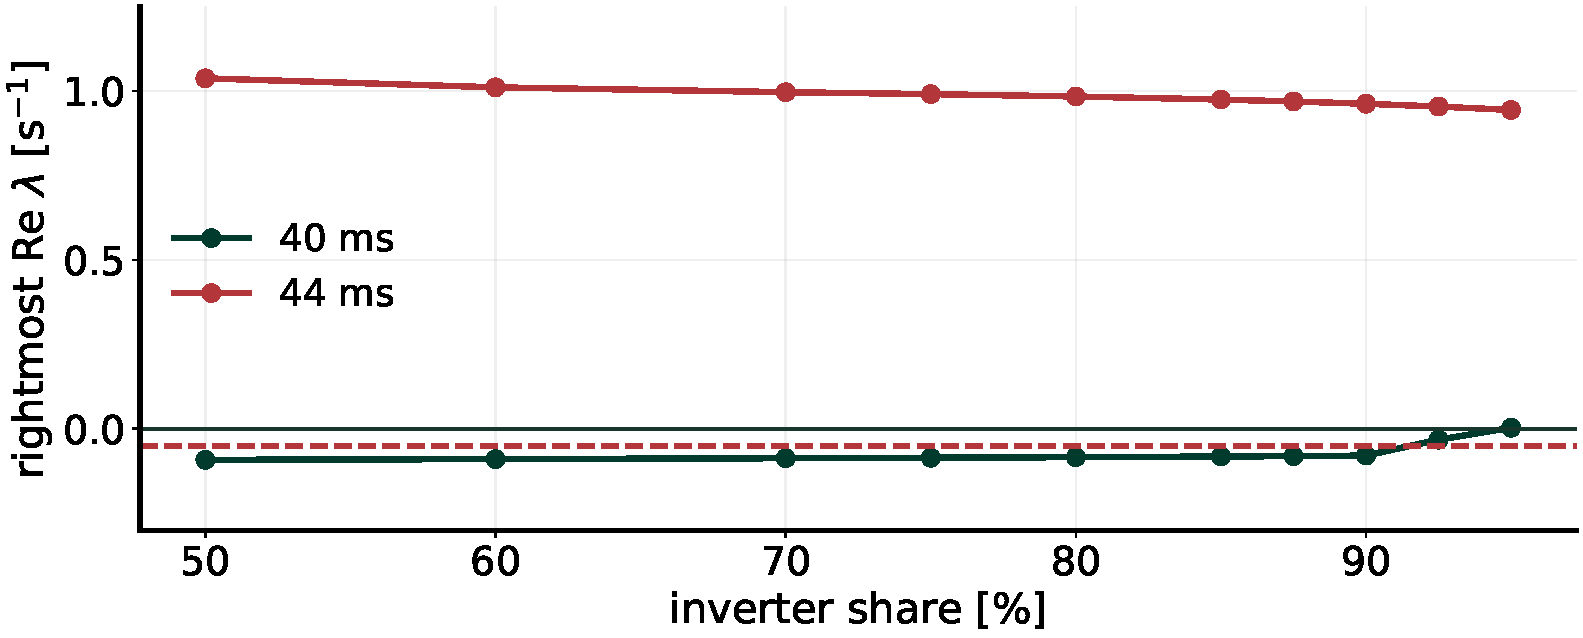
\includegraphics[width=268mm,height=92mm,keepaspectratio]{generated/figures/share_margin.pdf}\par
    {\fontsize{22pt}{25pt}\selectfont Rightmost root versus inverter share (exact delay): at 40 ms the margin holds up to 90\,\% share; at 44 ms the PLL family is unstable at every share from 50\,\%.\par}

  \end{PosterPanel}
\end{minipage}%
}%
\ifdefined\PosterFull
  \PosterSectionContent
  \let\PosterSectionFinish\relax
\else
  \def\PosterPageWidth{\PosterPreviewThreePageWidth}
  \def\PosterPageHeight{\PosterPreviewTopRowPageHeight}
  \def\PosterPreviewLeft{\PosterPreviewThreeLeft}
  \documentclass[final]{beamer}
% Fixed outer geometry for the IAS 2026 poster and its standalone previews.
% Edit this file only when changing the composition of the whole poster.
\def\PosterLayoutLoaded{1}
\newcommand{\PosterOuterMargin}{23mm}
\newcommand{\PosterColumnGap}{8mm}
\newcommand{\PosterRowGap}{4mm}
\newcommand{\PosterGridWidthMm}{868.4}
\newcommand{\PosterGridWidth}{\PosterGridWidthMm mm}
\newcommand{\PosterIdentityLeft}{8mm}
\newcommand{\PosterIdentityWidthMm}{898.4}
\newcommand{\PosterIdentityWidth}{\PosterIdentityWidthMm mm}
\newcommand{\PosterIdentityHeightMm}{54}
\newcommand{\PosterGreenHeightMm}{86}
\newcommand{\PosterHeaderHeightMm}{140}
\newcommand{\PosterHeaderHeight}{\PosterHeaderHeightMm mm}
\newcommand{\PosterGreenInset}{15mm}
\newcommand{\PosterHeaderTopOffset}{-3mm}
\newcommand{\PosterPhysicalPageWidthCm}{91.44}
\newcommand{\PosterPhysicalPageHeightCm}{106.68}

\newcommand{\PosterColWidth}{284.13mm}

\newcommand{\PosterRowHeight}{258mm}
\newcommand{\PosterRowHeightC}{352mm}
\newcommand{\PosterRowHeightA}{200mm}
% Module envelopes: width x height. Interior drawings remain local to each file.
\newcommand{\PosterOneWidth}{224mm}
\newcommand{\PosterTwoWidth}{412.4mm}
\newcommand{\PosterThreeWidth}{216mm}
\newcommand{\PosterTopRowHeight}{200mm}
\newcommand{\PosterStripHeight}{44mm}
\newcommand{\PosterFourHeight}{140mm}
\newcommand{\PosterHalfWidth}{430.2mm}
\newcommand{\PosterMiddleRowHeight}{140mm}
\newcommand{\PosterLowerRowHeight}{160mm}
\newcommand{\PosterBottomRowHeightMm}{84}
\newcommand{\PosterBottomRowHeight}{\PosterBottomRowHeightMm mm}

% Preview page sizes are centimetre numbers consumed by beamerposter.
\newcommand{\PosterPreviewTop}{6mm}
\newcommand{\PosterPreviewFullPageWidth}{\PosterPhysicalPageWidthCm}
\newcommand{\PosterPreviewWhitePageHeight}{8.0}
\newcommand{\PosterPreviewGreenPageHeight}{11.2}
\newcommand{\PosterPreviewTopRowPageHeight}{22.6}
\newcommand{\PosterPreviewStripPageHeight}{7.0}
\newcommand{\PosterPreviewFourPageHeight}{16.6}
\newcommand{\PosterPreviewMiddlePageHeight}{16.4}
\newcommand{\PosterPreviewLowerPageHeight}{18.6}
\newcommand{\PosterPreviewBottomPageHeight}{11.0}
\newcommand{\PosterPreviewOnePageWidth}{24.8}
\newcommand{\PosterPreviewTwoPageWidth}{43.6}
\newcommand{\PosterPreviewThreePageWidth}{23.84}
\newcommand{\PosterPreviewHalfPageWidth}{46.2}
\newcommand{\PosterPreviewOneLeft}{12mm}
\newcommand{\PosterPreviewTwoLeft}{11.8mm}
\newcommand{\PosterPreviewThreeLeft}{11.2mm}
\newcommand{\PosterPreviewHalfLeft}{15.9mm}

\usepackage[size=custom,width=\PosterPageWidth,height=\PosterPageHeight,scale=1.0]{beamerposter}
\usepackage{fontspec}
\usepackage{unicode-math}
\usepackage{amsmath,amssymb,mathtools}
\usepackage{graphicx}
\usepackage{tikz}
\usetikzlibrary{calc,positioning,shapes.geometric,shapes.misc,arrows.meta,patterns}
\usepackage{pgfplots}
\pgfplotsset{compat=1.18}
\usepackage{booktabs,tabularx,array}
\usepackage{ragged2e}
\usepackage[most]{tcolorbox}
\tcbuselibrary{skins,breakable}

% Shared visual roles and components, then scientific values used by the sections.
\input{poster_design_system.tex}
\input{generated/results.tex}
\input{generated/claims.tex}

\begin{document}

  \begin{frame}[t]
  \vspace*{\PosterPreviewTop}
  \noindent\hspace*{\PosterPreviewLeft}%
  \PosterSectionContent
  \end{frame}
  \def\PosterSectionFinish{\end{document}
}
\fi
\PosterSectionFinish
\par
\vspace{\PosterRowGap}

\noindent\hspace*{\PosterOuterMargin}%
% Collective-interaction version. Original poster preserved.
\long\def\PosterSectionContent{%
\begin{minipage}[t][\PosterRowHeight][t]{\PosterColWidth}\vspace{0pt}
  \begin{PosterPanel}{\PosterRowHeight}{4}{EXACT CLOSURE FACTORIZATION}

    {\FigureSize Open the ten PLLs, keep the whole grid:\par}
    {\fontsize{26pt}{31pt}\selectfont\color{IASBlue}\[
      G=C(sI-A_0)^{-1}B,\quad L_i=1-G_{ii}e^{-s\tau_i},\quad
      Q_{ij}=-\frac{G_{ij}e^{-s\tau_j}}{L_i}
    \]}\par\vspace{1mm}
    \vspace{-3mm}
    {\fontsize{32pt}{38pt}\selectfont\color{IASBlue}\[
      \boxed{\det\Delta=\det(sI-A_0)\prod_i L_i\cdot\det(I+Q)}
    \]}\par\vspace{1mm}
    \vspace{-3mm}
    {\fontsize{24pt}{29pt}\selectfont\color{IASBlue}\[
      \det(I+Q)=1-\!\sum_{i<j}p_{ij}+\!\sum Q_{ij}Q_{jk}Q_{ki}-\cdots,\quad p_{ij}=Q_{ij}Q_{ji}
    \]}\par\vspace{1mm}
    \vspace{-2mm}
    \noindent\begin{minipage}[c]{128mm}
      \begin{tikzpicture}[x=0.8mm,y=0.8mm,font=\fontsize{21pt}{23pt}\selectfont,
        nd/.style={circle,draw=IASDarkGreen,fill=IASPaleGreen,line width=1.1pt,minimum size=15mm,inner sep=0pt},
        hot/.style={circle,draw=IASVermillion,fill=IASPaleGold,line width=1.5pt,minimum size=15mm,inner sep=0pt},
        gr/.style={-{Stealth[length=3mm]},line width=1.1pt,color=IASGray},
        rd/.style={-{Stealth[length=3.5mm]},line width=2.2pt,color=IASVermillion}]
        \node[nd] (a) at (10,50) {$G_1$}; \node[hot] (b) at (70,50) {$G_2$}; \node[hot] (c) at (70,6) {$G_3$}; \node[nd] (d) at (10,6) {$G_4$};
        \draw[gr] (a)--(b); \draw[gr] (d)--(a); \draw[gr] (c)--(d); \draw[gr] (a)--(c); \draw[gr] (d)--(b);
        \draw[rd] ([xshift=-3mm]b.south)--([xshift=-3mm]c.north); \draw[rd] ([xshift=3mm]c.north)--([xshift=3mm]b.south);
        \node[align=center,font=\fontsize{19pt}{21pt}\selectfont\color{IASDarkText}] at (40,28) {network\\$K(s)$};
        \node[anchor=west,font=\fontsize{20pt}{22pt}\selectfont\color{IASVermillion}] at (76,28) {$p_{23}\!\to\!1$};
      \end{tikzpicture}
    \end{minipage}\hfill%
    \begin{minipage}[c]{136mm}
      \begin{tcolorbox}[colback=IASPaleGold,colframe=IASGold,boxrule=0.8pt,arc=1.5mm,left=2mm,right=2mm,top=1mm,bottom=1mm]
        {\fontsize{22pt}{25pt}\selectfont\textbf{IN WORDS} Delay drives $\det(I+Q)$ to zero while every $L_i$ stays away from zero: the failure belongs to a cycle, not to a device.\par}
      \end{tcolorbox}
    \end{minipage}\par

  \end{PosterPanel}
\end{minipage}%
}%
\ifdefined\PosterFull
  \PosterSectionContent
  \let\PosterSectionFinish\relax
\else
  \def\PosterPageWidth{\PosterPreviewFullPageWidth}
  \def\PosterPageHeight{\PosterPreviewFourPageHeight}
  \def\PosterPreviewLeft{\PosterOuterMargin}
  \documentclass[final]{beamer}
% Fixed outer geometry for the IAS 2026 poster and its standalone previews.
% Edit this file only when changing the composition of the whole poster.
\def\PosterLayoutLoaded{1}
\newcommand{\PosterOuterMargin}{23mm}
\newcommand{\PosterColumnGap}{8mm}
\newcommand{\PosterRowGap}{4mm}
\newcommand{\PosterGridWidthMm}{868.4}
\newcommand{\PosterGridWidth}{\PosterGridWidthMm mm}
\newcommand{\PosterIdentityLeft}{8mm}
\newcommand{\PosterIdentityWidthMm}{898.4}
\newcommand{\PosterIdentityWidth}{\PosterIdentityWidthMm mm}
\newcommand{\PosterIdentityHeightMm}{54}
\newcommand{\PosterGreenHeightMm}{86}
\newcommand{\PosterHeaderHeightMm}{140}
\newcommand{\PosterHeaderHeight}{\PosterHeaderHeightMm mm}
\newcommand{\PosterGreenInset}{15mm}
\newcommand{\PosterHeaderTopOffset}{-3mm}
\newcommand{\PosterPhysicalPageWidthCm}{91.44}
\newcommand{\PosterPhysicalPageHeightCm}{106.68}

\newcommand{\PosterColWidth}{284.13mm}

\newcommand{\PosterRowHeight}{258mm}
\newcommand{\PosterRowHeightC}{352mm}
\newcommand{\PosterRowHeightA}{200mm}
% Module envelopes: width x height. Interior drawings remain local to each file.
\newcommand{\PosterOneWidth}{224mm}
\newcommand{\PosterTwoWidth}{412.4mm}
\newcommand{\PosterThreeWidth}{216mm}
\newcommand{\PosterTopRowHeight}{200mm}
\newcommand{\PosterStripHeight}{44mm}
\newcommand{\PosterFourHeight}{140mm}
\newcommand{\PosterHalfWidth}{430.2mm}
\newcommand{\PosterMiddleRowHeight}{140mm}
\newcommand{\PosterLowerRowHeight}{160mm}
\newcommand{\PosterBottomRowHeightMm}{84}
\newcommand{\PosterBottomRowHeight}{\PosterBottomRowHeightMm mm}

% Preview page sizes are centimetre numbers consumed by beamerposter.
\newcommand{\PosterPreviewTop}{6mm}
\newcommand{\PosterPreviewFullPageWidth}{\PosterPhysicalPageWidthCm}
\newcommand{\PosterPreviewWhitePageHeight}{8.0}
\newcommand{\PosterPreviewGreenPageHeight}{11.2}
\newcommand{\PosterPreviewTopRowPageHeight}{22.6}
\newcommand{\PosterPreviewStripPageHeight}{7.0}
\newcommand{\PosterPreviewFourPageHeight}{16.6}
\newcommand{\PosterPreviewMiddlePageHeight}{16.4}
\newcommand{\PosterPreviewLowerPageHeight}{18.6}
\newcommand{\PosterPreviewBottomPageHeight}{11.0}
\newcommand{\PosterPreviewOnePageWidth}{24.8}
\newcommand{\PosterPreviewTwoPageWidth}{43.6}
\newcommand{\PosterPreviewThreePageWidth}{23.84}
\newcommand{\PosterPreviewHalfPageWidth}{46.2}
\newcommand{\PosterPreviewOneLeft}{12mm}
\newcommand{\PosterPreviewTwoLeft}{11.8mm}
\newcommand{\PosterPreviewThreeLeft}{11.2mm}
\newcommand{\PosterPreviewHalfLeft}{15.9mm}

\usepackage[size=custom,width=\PosterPageWidth,height=\PosterPageHeight,scale=1.0]{beamerposter}
\usepackage{fontspec}
\usepackage{unicode-math}
\usepackage{amsmath,amssymb,mathtools}
\usepackage{graphicx}
\usepackage{tikz}
\usetikzlibrary{calc,positioning,shapes.geometric,shapes.misc,arrows.meta,patterns}
\usepackage{pgfplots}
\pgfplotsset{compat=1.18}
\usepackage{booktabs,tabularx,array}
\usepackage{ragged2e}
\usepackage[most]{tcolorbox}
\tcbuselibrary{skins,breakable}

% Shared visual roles and components, then scientific values used by the sections.
\input{poster_design_system.tex}
\input{generated/results.tex}
\input{generated/claims.tex}

\begin{document}

  \begin{frame}[t]
  \vspace*{\PosterPreviewTop}
  \noindent\hspace*{\PosterPreviewLeft}%
  \PosterSectionContent
  \end{frame}
  \def\PosterSectionFinish{\end{document}
}
\fi
\PosterSectionFinish
\hspace{\PosterColumnGap}%
% Collective-interaction version. Original poster preserved.
\long\def\PosterSectionContent{%
\begin{minipage}[t][\PosterRowHeight][t]{\PosterColWidth}\vspace{0pt}
  \begin{PosterPanel}{\PosterRowHeight}{5}{EFFECTIVE DAMPING OPERATORS}

    {\FigureSize The controllers add a self-energy $\Pi(s)$ to the swing operator:\par}
    {\fontsize{25pt}{30pt}\selectfont\color{IASBlue}\[
      T(s)=s^{2}M+sD_0+L+\Pi(s)
    \]
    \[
      M_{\rm eff}=M+\frac{\Pi_e(s)-\Pi_e(0)}{s^{2}},\qquad
      D_{\rm eff}=D_0+\frac{\Pi_o(s)}{s}
    \]}\par\vspace{2.5mm}
    \vspace{-3mm}
    {\FigureSize Harmonic damping supplied to the generators, and what one PLL change does to it:\par}
    {\fontsize{27pt}{32pt}\selectfont\color{IASBlue}\[
      D_H(\Omega)=\mathrm{Herm}\,Z(\mathrm{j}\Omega),\qquad
      \delta D_H=\tfrac12\,(a\,v^{*}+v\,a^{*})
    \]}\par\vspace{2.5mm}
    \vspace{-4mm}
    \begin{center}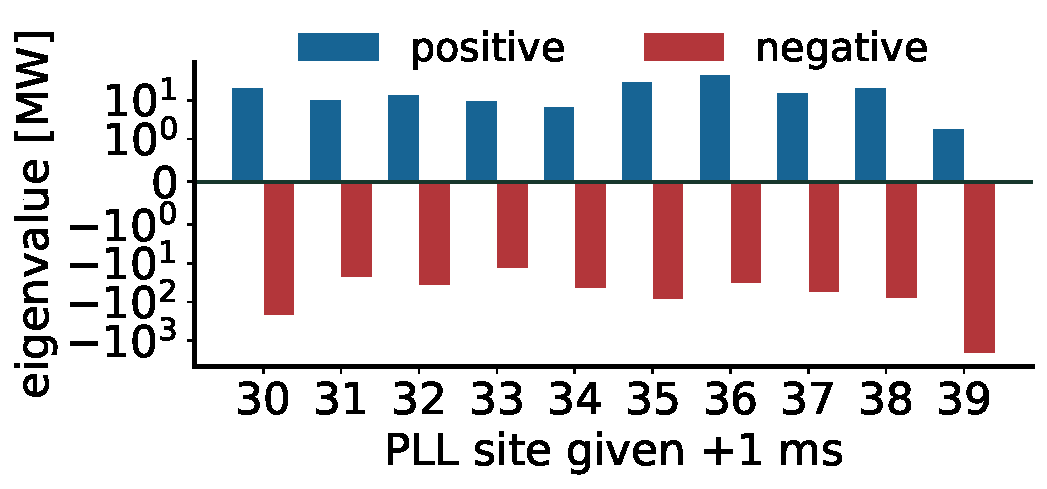
\includegraphics[width=262mm,height=78mm,keepaspectratio]{generated/figures/rank_two2.pdf}\end{center}
    \vspace{-1mm}
    {\fontsize{22pt}{25pt}\selectfont IEEE-39, $+1$ ms at each PLL, 5 Hz: one positive and one negative eigenvalue (60 of 60 checks).\par}
    \vspace{1mm}
    \begin{tcolorbox}[colback=IASPaleGold,colframe=IASGold,boxrule=0.8pt,arc=1.5mm,left=2mm,right=2mm,top=1mm,bottom=1mm]
      {\fontsize{22pt}{25pt}\selectfont\textbf{IN WORDS} A local change moves damping up along one network path and down along another. Damping at one frequency is not a stability test.\par}
    \end{tcolorbox}

  \end{PosterPanel}
\end{minipage}%
}%
\ifdefined\PosterFull
  \PosterSectionContent
  \let\PosterSectionFinish\relax
\else
  \def\PosterPageWidth{\PosterPreviewHalfPageWidth}
  \def\PosterPageHeight{\PosterPreviewMiddlePageHeight}
  \def\PosterPreviewLeft{\PosterPreviewHalfLeft}
  \documentclass[final]{beamer}
% Fixed outer geometry for the IAS 2026 poster and its standalone previews.
% Edit this file only when changing the composition of the whole poster.
\def\PosterLayoutLoaded{1}
\newcommand{\PosterOuterMargin}{23mm}
\newcommand{\PosterColumnGap}{8mm}
\newcommand{\PosterRowGap}{4mm}
\newcommand{\PosterGridWidthMm}{868.4}
\newcommand{\PosterGridWidth}{\PosterGridWidthMm mm}
\newcommand{\PosterIdentityLeft}{8mm}
\newcommand{\PosterIdentityWidthMm}{898.4}
\newcommand{\PosterIdentityWidth}{\PosterIdentityWidthMm mm}
\newcommand{\PosterIdentityHeightMm}{54}
\newcommand{\PosterGreenHeightMm}{86}
\newcommand{\PosterHeaderHeightMm}{140}
\newcommand{\PosterHeaderHeight}{\PosterHeaderHeightMm mm}
\newcommand{\PosterGreenInset}{15mm}
\newcommand{\PosterHeaderTopOffset}{-3mm}
\newcommand{\PosterPhysicalPageWidthCm}{91.44}
\newcommand{\PosterPhysicalPageHeightCm}{106.68}

\newcommand{\PosterColWidth}{284.13mm}

\newcommand{\PosterRowHeight}{258mm}
\newcommand{\PosterRowHeightC}{352mm}
\newcommand{\PosterRowHeightA}{200mm}
% Module envelopes: width x height. Interior drawings remain local to each file.
\newcommand{\PosterOneWidth}{224mm}
\newcommand{\PosterTwoWidth}{412.4mm}
\newcommand{\PosterThreeWidth}{216mm}
\newcommand{\PosterTopRowHeight}{200mm}
\newcommand{\PosterStripHeight}{44mm}
\newcommand{\PosterFourHeight}{140mm}
\newcommand{\PosterHalfWidth}{430.2mm}
\newcommand{\PosterMiddleRowHeight}{140mm}
\newcommand{\PosterLowerRowHeight}{160mm}
\newcommand{\PosterBottomRowHeightMm}{84}
\newcommand{\PosterBottomRowHeight}{\PosterBottomRowHeightMm mm}

% Preview page sizes are centimetre numbers consumed by beamerposter.
\newcommand{\PosterPreviewTop}{6mm}
\newcommand{\PosterPreviewFullPageWidth}{\PosterPhysicalPageWidthCm}
\newcommand{\PosterPreviewWhitePageHeight}{8.0}
\newcommand{\PosterPreviewGreenPageHeight}{11.2}
\newcommand{\PosterPreviewTopRowPageHeight}{22.6}
\newcommand{\PosterPreviewStripPageHeight}{7.0}
\newcommand{\PosterPreviewFourPageHeight}{16.6}
\newcommand{\PosterPreviewMiddlePageHeight}{16.4}
\newcommand{\PosterPreviewLowerPageHeight}{18.6}
\newcommand{\PosterPreviewBottomPageHeight}{11.0}
\newcommand{\PosterPreviewOnePageWidth}{24.8}
\newcommand{\PosterPreviewTwoPageWidth}{43.6}
\newcommand{\PosterPreviewThreePageWidth}{23.84}
\newcommand{\PosterPreviewHalfPageWidth}{46.2}
\newcommand{\PosterPreviewOneLeft}{12mm}
\newcommand{\PosterPreviewTwoLeft}{11.8mm}
\newcommand{\PosterPreviewThreeLeft}{11.2mm}
\newcommand{\PosterPreviewHalfLeft}{15.9mm}

\usepackage[size=custom,width=\PosterPageWidth,height=\PosterPageHeight,scale=1.0]{beamerposter}
\usepackage{fontspec}
\usepackage{unicode-math}
\usepackage{amsmath,amssymb,mathtools}
\usepackage{graphicx}
\usepackage{tikz}
\usetikzlibrary{calc,positioning,shapes.geometric,shapes.misc,arrows.meta,patterns}
\usepackage{pgfplots}
\pgfplotsset{compat=1.18}
\usepackage{booktabs,tabularx,array}
\usepackage{ragged2e}
\usepackage[most]{tcolorbox}
\tcbuselibrary{skins,breakable}

% Shared visual roles and components, then scientific values used by the sections.
\input{poster_design_system.tex}
\input{generated/results.tex}
\input{generated/claims.tex}

\begin{document}

  \begin{frame}[t]
  \vspace*{\PosterPreviewTop}
  \noindent\hspace*{\PosterPreviewLeft}%
  \PosterSectionContent
  \end{frame}
  \def\PosterSectionFinish{\end{document}
}
\fi
\PosterSectionFinish
\hspace{\PosterColumnGap}%
% Collective-interaction version. Original poster preserved.
\long\def\PosterSectionContent{%
\begin{minipage}[t][\PosterRowHeight][t]{\PosterColWidth}\vspace{0pt}
  \begin{PosterPanel}{\PosterRowHeight}{6}{EXACT PLL GAIN SYNTHESIS}

    {\FigureSize \textbf{Target mode} $\lambda=\alpha+\mathrm{j}\omega$, right vector $q$, $y=G(\lambda)q$:\par}
    {\fontsize{25pt}{30pt}\selectfont\color{IASBlue}\[
      W_i=\frac{\lambda^{2}(1+t_f\lambda)e^{\lambda\tau_i}q_i}{y_i},\quad
      k_{p,i}=\frac{\mathrm{Im}W_i}{\omega},\quad
      k_{I,i}=\mathrm{Re}W_i-\alpha k_{p,i}
    \]}\par\vspace{1mm}
    \vspace{-4mm}
    {\FigureSize \textbf{Delay grows by $h$, keep $\lambda$} (exact transport):\par}
    {\fontsize{29pt}{34pt}\selectfont\color{IASBlue}\[
      \boxed{k_p(h)\lambda+k_I(h)=(k_p\lambda+k_I)\,e^{\lambda h}}
    \]}\par\vspace{1mm}
    \vspace{-4mm}
    {\FigureSize \textbf{Price paid by every other mode} $\mu$:\par}
    {\fontsize{27pt}{32pt}\selectfont\color{IASBlue}\[
      \frac{d\mu}{dh}=-k_p(\mu-\lambda)(\mu-\bar\lambda)\frac{\partial\mu}{\partial k_I},\quad
      \frac{\partial\mu}{\partial k_I}=-\frac{\ell^{H}Z_{k_I}r}{\ell^{H}Z_{s}r}
    \]}\par\vspace{1mm}
    \vspace{-4mm}
    {\fontsize{22pt}{25pt}\selectfont \textbf{Rule (fixed in advance):} among modes predicted safe, protect the one that keeps the most $k_I$. 9-bus bank: $+0.886\to-0.131\ \mathrm{s^{-1}}$.\par}
    \vspace{1mm}
    \begin{tcolorbox}[colback=IASPaleGold,colframe=IASGold,boxrule=0.8pt,arc=1.5mm,left=2mm,right=2mm,top=1mm,bottom=1mm]
      {\fontsize{22pt}{25pt}\selectfont\textbf{IN WORDS} PLL: quadratic factor. Grid: residue.\par}
    \end{tcolorbox}

  \end{PosterPanel}
\end{minipage}%
}%
\ifdefined\PosterFull
  \PosterSectionContent
  \let\PosterSectionFinish\relax
\else
  \def\PosterPageWidth{\PosterPreviewHalfPageWidth}
  \def\PosterPageHeight{\PosterPreviewMiddlePageHeight}
  \def\PosterPreviewLeft{\PosterPreviewHalfLeft}
  \documentclass[final]{beamer}
% Fixed outer geometry for the IAS 2026 poster and its standalone previews.
% Edit this file only when changing the composition of the whole poster.
\def\PosterLayoutLoaded{1}
\newcommand{\PosterOuterMargin}{23mm}
\newcommand{\PosterColumnGap}{8mm}
\newcommand{\PosterRowGap}{4mm}
\newcommand{\PosterGridWidthMm}{868.4}
\newcommand{\PosterGridWidth}{\PosterGridWidthMm mm}
\newcommand{\PosterIdentityLeft}{8mm}
\newcommand{\PosterIdentityWidthMm}{898.4}
\newcommand{\PosterIdentityWidth}{\PosterIdentityWidthMm mm}
\newcommand{\PosterIdentityHeightMm}{54}
\newcommand{\PosterGreenHeightMm}{86}
\newcommand{\PosterHeaderHeightMm}{140}
\newcommand{\PosterHeaderHeight}{\PosterHeaderHeightMm mm}
\newcommand{\PosterGreenInset}{15mm}
\newcommand{\PosterHeaderTopOffset}{-3mm}
\newcommand{\PosterPhysicalPageWidthCm}{91.44}
\newcommand{\PosterPhysicalPageHeightCm}{106.68}

\newcommand{\PosterColWidth}{284.13mm}

\newcommand{\PosterRowHeight}{258mm}
\newcommand{\PosterRowHeightC}{352mm}
\newcommand{\PosterRowHeightA}{200mm}
% Module envelopes: width x height. Interior drawings remain local to each file.
\newcommand{\PosterOneWidth}{224mm}
\newcommand{\PosterTwoWidth}{412.4mm}
\newcommand{\PosterThreeWidth}{216mm}
\newcommand{\PosterTopRowHeight}{200mm}
\newcommand{\PosterStripHeight}{44mm}
\newcommand{\PosterFourHeight}{140mm}
\newcommand{\PosterHalfWidth}{430.2mm}
\newcommand{\PosterMiddleRowHeight}{140mm}
\newcommand{\PosterLowerRowHeight}{160mm}
\newcommand{\PosterBottomRowHeightMm}{84}
\newcommand{\PosterBottomRowHeight}{\PosterBottomRowHeightMm mm}

% Preview page sizes are centimetre numbers consumed by beamerposter.
\newcommand{\PosterPreviewTop}{6mm}
\newcommand{\PosterPreviewFullPageWidth}{\PosterPhysicalPageWidthCm}
\newcommand{\PosterPreviewWhitePageHeight}{8.0}
\newcommand{\PosterPreviewGreenPageHeight}{11.2}
\newcommand{\PosterPreviewTopRowPageHeight}{22.6}
\newcommand{\PosterPreviewStripPageHeight}{7.0}
\newcommand{\PosterPreviewFourPageHeight}{16.6}
\newcommand{\PosterPreviewMiddlePageHeight}{16.4}
\newcommand{\PosterPreviewLowerPageHeight}{18.6}
\newcommand{\PosterPreviewBottomPageHeight}{11.0}
\newcommand{\PosterPreviewOnePageWidth}{24.8}
\newcommand{\PosterPreviewTwoPageWidth}{43.6}
\newcommand{\PosterPreviewThreePageWidth}{23.84}
\newcommand{\PosterPreviewHalfPageWidth}{46.2}
\newcommand{\PosterPreviewOneLeft}{12mm}
\newcommand{\PosterPreviewTwoLeft}{11.8mm}
\newcommand{\PosterPreviewThreeLeft}{11.2mm}
\newcommand{\PosterPreviewHalfLeft}{15.9mm}

\usepackage[size=custom,width=\PosterPageWidth,height=\PosterPageHeight,scale=1.0]{beamerposter}
\usepackage{fontspec}
\usepackage{unicode-math}
\usepackage{amsmath,amssymb,mathtools}
\usepackage{graphicx}
\usepackage{tikz}
\usetikzlibrary{calc,positioning,shapes.geometric,shapes.misc,arrows.meta,patterns}
\usepackage{pgfplots}
\pgfplotsset{compat=1.18}
\usepackage{booktabs,tabularx,array}
\usepackage{ragged2e}
\usepackage[most]{tcolorbox}
\tcbuselibrary{skins,breakable}

% Shared visual roles and components, then scientific values used by the sections.
\input{poster_design_system.tex}
\input{generated/results.tex}
\input{generated/claims.tex}

\begin{document}

  \begin{frame}[t]
  \vspace*{\PosterPreviewTop}
  \noindent\hspace*{\PosterPreviewLeft}%
  \PosterSectionContent
  \end{frame}
  \def\PosterSectionFinish{\end{document}
}
\fi
\PosterSectionFinish
\par
\vspace{\PosterRowGap}

\noindent\hspace*{\PosterOuterMargin}%
% Collective-interaction version. Original poster preserved.
\long\def\PosterSectionContent{%
\begin{minipage}[t][\PosterRowHeightC][t]{\PosterColWidth}\vspace{0pt}
  \begin{PosterPanel}{\PosterRowHeightC}{7}{CO-DESIGN ALGORITHM}

    \noindent\begin{minipage}[t]{120mm}\vspace{0pt}
      \begin{tikzpicture}[x=1mm,y=1mm,font=\fontsize{19pt}{21pt}\selectfont,
        st/.style={draw=IASDarkGreen,fill=IASPaleGreen,line width=1pt,rounded corners=1.2mm,minimum height=15mm,text width=108mm,align=left,inner sep=1.2mm},
        ar/.style={-{Stealth[length=2.6mm]},line width=1.1pt,color=IASDarkGreen}]
        \node[st] (s1) at (0,0) {\textbf{1} open PLLs, keep grid: $G(s)$};
        \node[st] (s2) at (0,-19) {\textbf{2} diagnose: $\mathrm{eig}(Q)$, cycles $p_{ij}$};
        \node[st] (s3) at (0,-38) {\textbf{3} gain map or transport\\$\lambda\mapsto(k_p,k_I)$};
        \node[st] (s4) at (0,-57) {\textbf{4} predict: $\min\tfrac12|\delta|^2$\\s.t. $\mathrm{Re}\lambda_r+g_r\!\cdot\!\delta\le-\sigma$};
        \node[st,fill=IASPaleGold] (s5) at (0,-76) {\textbf{5} correct: exact spectrum,\\shrink step if worse};
        \node[st] (s6) at (0,-95) {\textbf{6} verify: roots + five events};
        \foreach \a/\b in {s1/s2,s2/s3,s3/s4,s4/s5,s5/s6}{\draw[ar] (\a) -- (\b);}
        \draw[ar,color=IASVermillion] (s5.east) -- ++(5,0) |- (s4.east);
      \end{tikzpicture}
      \vspace{4mm}
      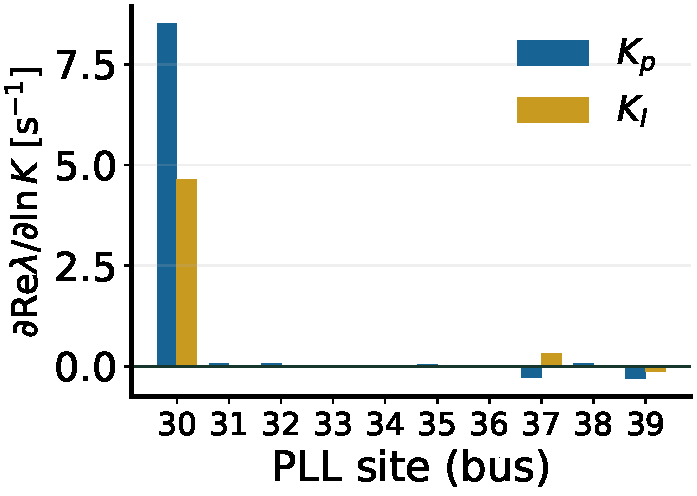
\includegraphics[width=118mm,height=84mm,keepaspectratio]{generated/figures/authority.pdf}\par
      {\fontsize{20pt}{23pt}\selectfont Leading 44 ms root: authority sits at site 30 (8.5\,s$^{-1}$ per $\ln K_p$), not at the cycle pair 35--36 ($\le0.05$).\par}
    \end{minipage}\hfill%
    \begin{minipage}[t]{146mm}\vspace{0pt}
      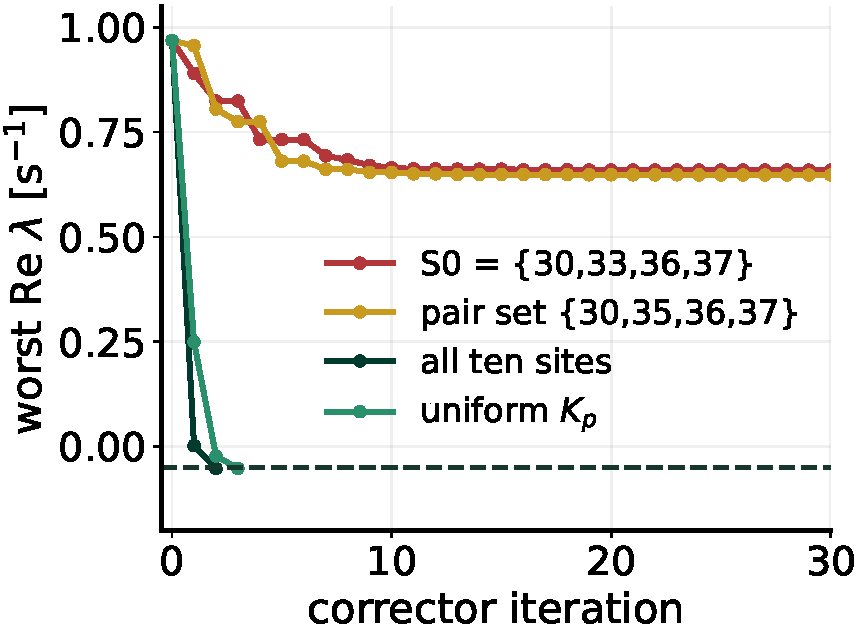
\includegraphics[width=146mm,height=108mm,keepaspectratio]{generated/figures/repair_curve.pdf}\par
      {\fontsize{20pt}{23pt}\selectfont Worst root per iteration, 44 ms.\par}
      \vspace{1mm}
      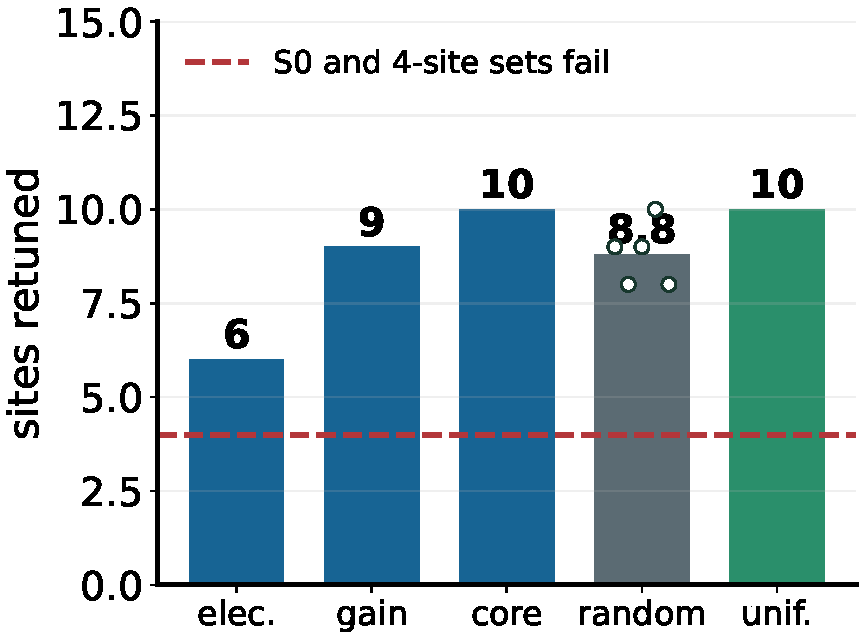
\includegraphics[width=146mm,height=108mm,keepaspectratio]{generated/figures/support_scan.pdf}\par
      {\fontsize{20pt}{23pt}\selectfont Sites retuned until the margin holds.\par}
    \end{minipage}\par
    \vspace{1mm}
    {\fontsize{22pt}{25pt}\selectfont \textbf{$S_0=\{30,33,36,37\}$ fails} ($K_I$, $K_p$, joint); so does every four-site set. One common $K_p$ cut of 14\,\% restores the margin.\par}

  \end{PosterPanel}
\end{minipage}%
}%
\ifdefined\PosterFull
  \PosterSectionContent
  \let\PosterSectionFinish\relax
\else
  \def\PosterPageWidth{\PosterPreviewHalfPageWidth}
  \def\PosterPageHeight{\PosterPreviewLowerPageHeight}
  \def\PosterPreviewLeft{\PosterPreviewHalfLeft}
  \documentclass[final]{beamer}
% Fixed outer geometry for the IAS 2026 poster and its standalone previews.
% Edit this file only when changing the composition of the whole poster.
\def\PosterLayoutLoaded{1}
\newcommand{\PosterOuterMargin}{23mm}
\newcommand{\PosterColumnGap}{8mm}
\newcommand{\PosterRowGap}{4mm}
\newcommand{\PosterGridWidthMm}{868.4}
\newcommand{\PosterGridWidth}{\PosterGridWidthMm mm}
\newcommand{\PosterIdentityLeft}{8mm}
\newcommand{\PosterIdentityWidthMm}{898.4}
\newcommand{\PosterIdentityWidth}{\PosterIdentityWidthMm mm}
\newcommand{\PosterIdentityHeightMm}{54}
\newcommand{\PosterGreenHeightMm}{86}
\newcommand{\PosterHeaderHeightMm}{140}
\newcommand{\PosterHeaderHeight}{\PosterHeaderHeightMm mm}
\newcommand{\PosterGreenInset}{15mm}
\newcommand{\PosterHeaderTopOffset}{-3mm}
\newcommand{\PosterPhysicalPageWidthCm}{91.44}
\newcommand{\PosterPhysicalPageHeightCm}{106.68}

\newcommand{\PosterColWidth}{284.13mm}

\newcommand{\PosterRowHeight}{258mm}
\newcommand{\PosterRowHeightC}{352mm}
\newcommand{\PosterRowHeightA}{200mm}
% Module envelopes: width x height. Interior drawings remain local to each file.
\newcommand{\PosterOneWidth}{224mm}
\newcommand{\PosterTwoWidth}{412.4mm}
\newcommand{\PosterThreeWidth}{216mm}
\newcommand{\PosterTopRowHeight}{200mm}
\newcommand{\PosterStripHeight}{44mm}
\newcommand{\PosterFourHeight}{140mm}
\newcommand{\PosterHalfWidth}{430.2mm}
\newcommand{\PosterMiddleRowHeight}{140mm}
\newcommand{\PosterLowerRowHeight}{160mm}
\newcommand{\PosterBottomRowHeightMm}{84}
\newcommand{\PosterBottomRowHeight}{\PosterBottomRowHeightMm mm}

% Preview page sizes are centimetre numbers consumed by beamerposter.
\newcommand{\PosterPreviewTop}{6mm}
\newcommand{\PosterPreviewFullPageWidth}{\PosterPhysicalPageWidthCm}
\newcommand{\PosterPreviewWhitePageHeight}{8.0}
\newcommand{\PosterPreviewGreenPageHeight}{11.2}
\newcommand{\PosterPreviewTopRowPageHeight}{22.6}
\newcommand{\PosterPreviewStripPageHeight}{7.0}
\newcommand{\PosterPreviewFourPageHeight}{16.6}
\newcommand{\PosterPreviewMiddlePageHeight}{16.4}
\newcommand{\PosterPreviewLowerPageHeight}{18.6}
\newcommand{\PosterPreviewBottomPageHeight}{11.0}
\newcommand{\PosterPreviewOnePageWidth}{24.8}
\newcommand{\PosterPreviewTwoPageWidth}{43.6}
\newcommand{\PosterPreviewThreePageWidth}{23.84}
\newcommand{\PosterPreviewHalfPageWidth}{46.2}
\newcommand{\PosterPreviewOneLeft}{12mm}
\newcommand{\PosterPreviewTwoLeft}{11.8mm}
\newcommand{\PosterPreviewThreeLeft}{11.2mm}
\newcommand{\PosterPreviewHalfLeft}{15.9mm}

\usepackage[size=custom,width=\PosterPageWidth,height=\PosterPageHeight,scale=1.0]{beamerposter}
\usepackage{fontspec}
\usepackage{unicode-math}
\usepackage{amsmath,amssymb,mathtools}
\usepackage{graphicx}
\usepackage{tikz}
\usetikzlibrary{calc,positioning,shapes.geometric,shapes.misc,arrows.meta,patterns}
\usepackage{pgfplots}
\pgfplotsset{compat=1.18}
\usepackage{booktabs,tabularx,array}
\usepackage{ragged2e}
\usepackage[most]{tcolorbox}
\tcbuselibrary{skins,breakable}

% Shared visual roles and components, then scientific values used by the sections.
\input{poster_design_system.tex}
\input{generated/results.tex}
\input{generated/claims.tex}

\begin{document}

  \begin{frame}[t]
  \vspace*{\PosterPreviewTop}
  \noindent\hspace*{\PosterPreviewLeft}%
  \PosterSectionContent
  \end{frame}
  \def\PosterSectionFinish{\end{document}
}
\fi
\PosterSectionFinish
\hspace{\PosterColumnGap}%
% Collective-interaction version. Original poster preserved.
\long\def\PosterSectionContent{%
\begin{minipage}[t][\PosterRowHeightC][t]{\PosterColWidth}\vspace{0pt}
  \begin{PosterPanel}{\PosterRowHeightC}{8}{FULL-GRID DELAY EVIDENCE}

    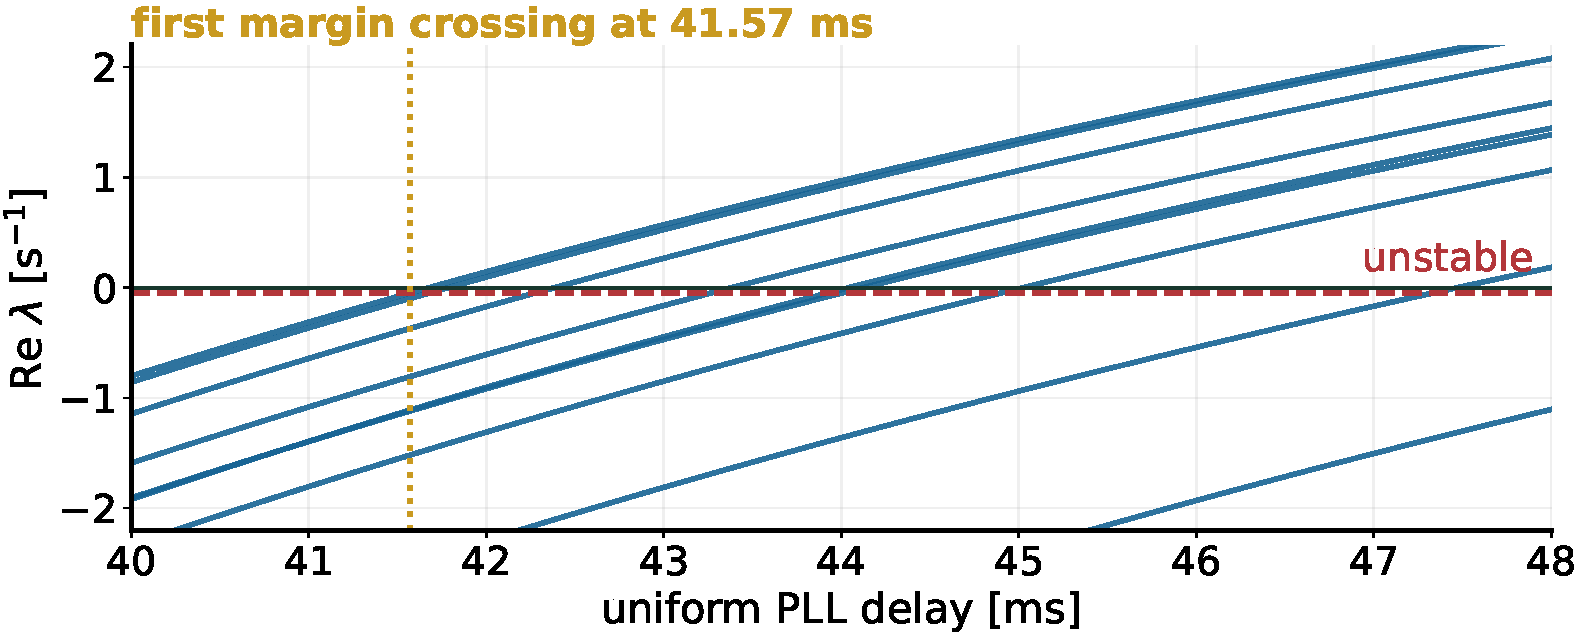
\includegraphics[width=268mm,height=108mm,keepaspectratio]{generated/figures/delay_locus.pdf}\par
    {\fontsize{21pt}{24pt}\selectfont Exact-delay roots of the 4.5--5 Hz PLL family. Unstable roots: 0, 0, 4, 6, 8 at 40, 41, 42, 43, 44 ms. Absent from the all-SG grid (modes stop at 1.5 Hz).\par}
    \vspace{1mm}
    \noindent\begin{minipage}[t]{130mm}\vspace{0pt}
      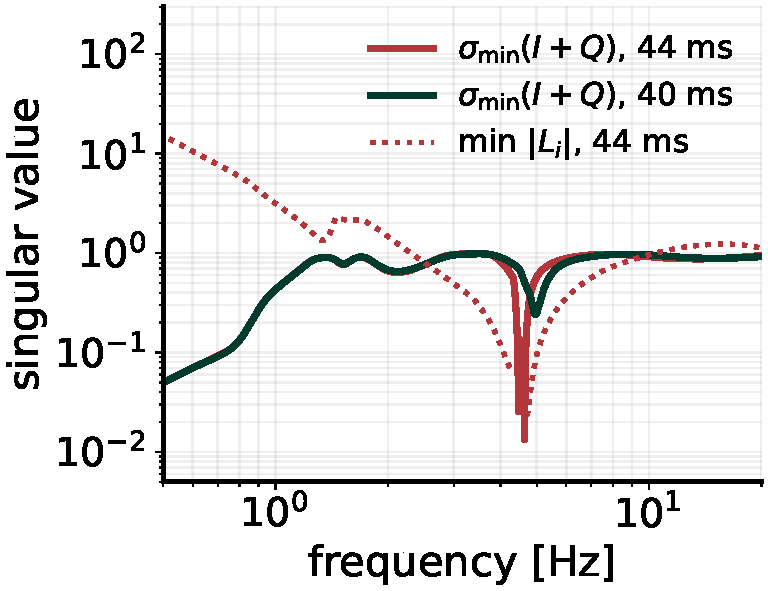
\includegraphics[width=130mm,height=100mm,keepaspectratio]{generated/figures/closure_scan.pdf}\par
    \end{minipage}\hfill%
    \begin{minipage}[t]{136mm}\vspace{0pt}
      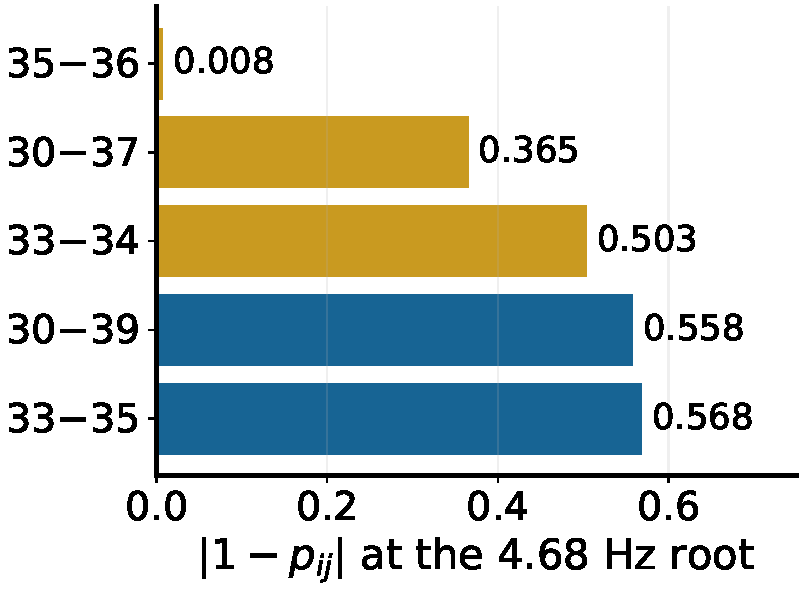
\includegraphics[width=136mm,height=100mm,keepaspectratio]{generated/figures/pair_cycles.pdf}\par
    \end{minipage}\par
    {\fontsize{21pt}{24pt}\selectfont $\sigma_{\min}(I+Q)$ dips at 4.7 Hz while local factors stay regular. Gold: predicted pairs. Closest cycles: 35$-$36 ($0.008$), 33$-$34, 36$-$37; the predicted pairs are the three strongest electrical couplings.\par}

    \vspace{2mm}
    {\fontsize{21pt}{25pt}\selectfont
    \begin{tabular}{@{}lccccccc@{}}
      \textbf{delay [ms]} & 40 & 41 & 42 & 43 & 44 & 46 & 48\\\hline
      unstable roots & 0 & 0 & 4 & 6 & 8 & 14 & 16\\
      beyond $-0.05$ & 0 & 0 & 4 & 6 & 10 & 14 & 16\\
    \end{tabular}\par}
    {\fontsize{20pt}{23pt}\selectfont Full-spectrum argument-principle counts (floating point, validated against eigenvalues at zero delay).\par}

  \end{PosterPanel}
\end{minipage}%
}%
\ifdefined\PosterFull
  \PosterSectionContent
  \let\PosterSectionFinish\relax
\else
  \def\PosterPageWidth{\PosterPreviewHalfPageWidth}
  \def\PosterPageHeight{\PosterPreviewLowerPageHeight}
  \def\PosterPreviewLeft{\PosterPreviewHalfLeft}
  \documentclass[final]{beamer}
% Fixed outer geometry for the IAS 2026 poster and its standalone previews.
% Edit this file only when changing the composition of the whole poster.
\def\PosterLayoutLoaded{1}
\newcommand{\PosterOuterMargin}{23mm}
\newcommand{\PosterColumnGap}{8mm}
\newcommand{\PosterRowGap}{4mm}
\newcommand{\PosterGridWidthMm}{868.4}
\newcommand{\PosterGridWidth}{\PosterGridWidthMm mm}
\newcommand{\PosterIdentityLeft}{8mm}
\newcommand{\PosterIdentityWidthMm}{898.4}
\newcommand{\PosterIdentityWidth}{\PosterIdentityWidthMm mm}
\newcommand{\PosterIdentityHeightMm}{54}
\newcommand{\PosterGreenHeightMm}{86}
\newcommand{\PosterHeaderHeightMm}{140}
\newcommand{\PosterHeaderHeight}{\PosterHeaderHeightMm mm}
\newcommand{\PosterGreenInset}{15mm}
\newcommand{\PosterHeaderTopOffset}{-3mm}
\newcommand{\PosterPhysicalPageWidthCm}{91.44}
\newcommand{\PosterPhysicalPageHeightCm}{106.68}

\newcommand{\PosterColWidth}{284.13mm}

\newcommand{\PosterRowHeight}{258mm}
\newcommand{\PosterRowHeightC}{352mm}
\newcommand{\PosterRowHeightA}{200mm}
% Module envelopes: width x height. Interior drawings remain local to each file.
\newcommand{\PosterOneWidth}{224mm}
\newcommand{\PosterTwoWidth}{412.4mm}
\newcommand{\PosterThreeWidth}{216mm}
\newcommand{\PosterTopRowHeight}{200mm}
\newcommand{\PosterStripHeight}{44mm}
\newcommand{\PosterFourHeight}{140mm}
\newcommand{\PosterHalfWidth}{430.2mm}
\newcommand{\PosterMiddleRowHeight}{140mm}
\newcommand{\PosterLowerRowHeight}{160mm}
\newcommand{\PosterBottomRowHeightMm}{84}
\newcommand{\PosterBottomRowHeight}{\PosterBottomRowHeightMm mm}

% Preview page sizes are centimetre numbers consumed by beamerposter.
\newcommand{\PosterPreviewTop}{6mm}
\newcommand{\PosterPreviewFullPageWidth}{\PosterPhysicalPageWidthCm}
\newcommand{\PosterPreviewWhitePageHeight}{8.0}
\newcommand{\PosterPreviewGreenPageHeight}{11.2}
\newcommand{\PosterPreviewTopRowPageHeight}{22.6}
\newcommand{\PosterPreviewStripPageHeight}{7.0}
\newcommand{\PosterPreviewFourPageHeight}{16.6}
\newcommand{\PosterPreviewMiddlePageHeight}{16.4}
\newcommand{\PosterPreviewLowerPageHeight}{18.6}
\newcommand{\PosterPreviewBottomPageHeight}{11.0}
\newcommand{\PosterPreviewOnePageWidth}{24.8}
\newcommand{\PosterPreviewTwoPageWidth}{43.6}
\newcommand{\PosterPreviewThreePageWidth}{23.84}
\newcommand{\PosterPreviewHalfPageWidth}{46.2}
\newcommand{\PosterPreviewOneLeft}{12mm}
\newcommand{\PosterPreviewTwoLeft}{11.8mm}
\newcommand{\PosterPreviewThreeLeft}{11.2mm}
\newcommand{\PosterPreviewHalfLeft}{15.9mm}

\usepackage[size=custom,width=\PosterPageWidth,height=\PosterPageHeight,scale=1.0]{beamerposter}
\usepackage{fontspec}
\usepackage{unicode-math}
\usepackage{amsmath,amssymb,mathtools}
\usepackage{graphicx}
\usepackage{tikz}
\usetikzlibrary{calc,positioning,shapes.geometric,shapes.misc,arrows.meta,patterns}
\usepackage{pgfplots}
\pgfplotsset{compat=1.18}
\usepackage{booktabs,tabularx,array}
\usepackage{ragged2e}
\usepackage[most]{tcolorbox}
\tcbuselibrary{skins,breakable}

% Shared visual roles and components, then scientific values used by the sections.
\input{poster_design_system.tex}
\input{generated/results.tex}
\input{generated/claims.tex}

\begin{document}

  \begin{frame}[t]
  \vspace*{\PosterPreviewTop}
  \noindent\hspace*{\PosterPreviewLeft}%
  \PosterSectionContent
  \end{frame}
  \def\PosterSectionFinish{\end{document}
}
\fi
\PosterSectionFinish
\hspace{\PosterColumnGap}%
% Collective-interaction version. Original poster preserved.
\long\def\PosterSectionContent{%
\begin{minipage}[t][\PosterRowHeightC][t]{\PosterColWidth}\vspace{0pt}
  \begin{PosterPanel}{\PosterRowHeightC}{9}{NONLINEAR CHECKS AND LIMITS}

    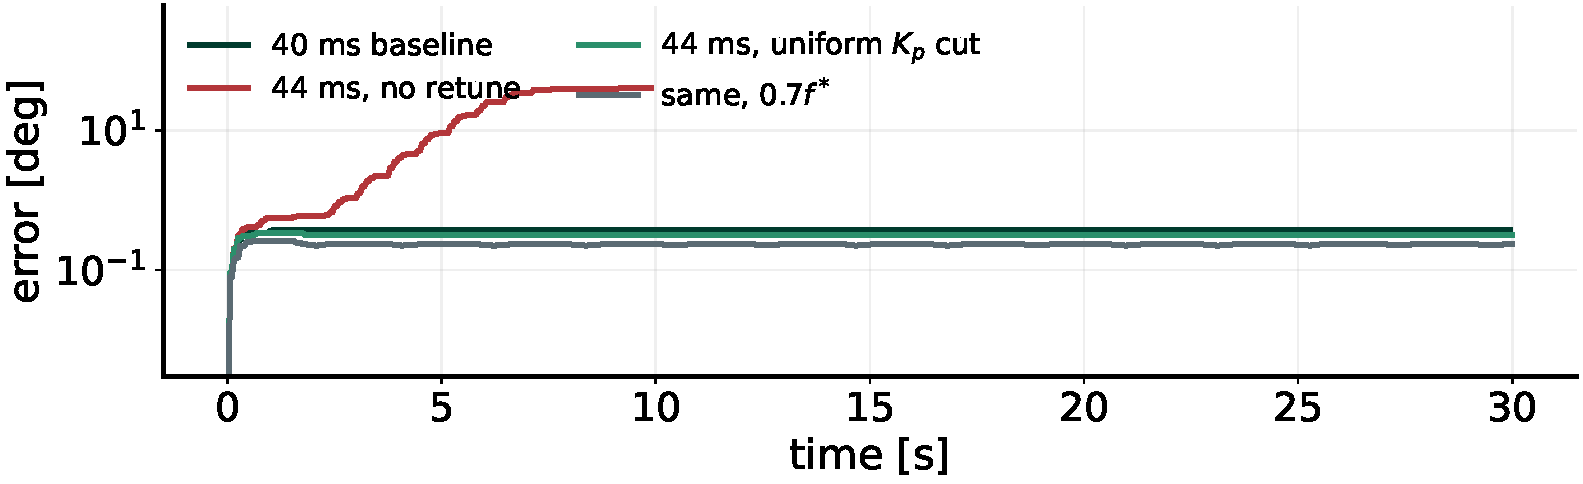
\includegraphics[width=268mm,height=82mm,keepaspectratio]{generated/figures/forced.pdf}\par
    {\fontsize{20pt}{23pt}\selectfont Forced response, 5 MW at bus 29, $f^{*}=4.65$ Hz (Julia, exact delay).\par}
    \vspace{0.5mm}
    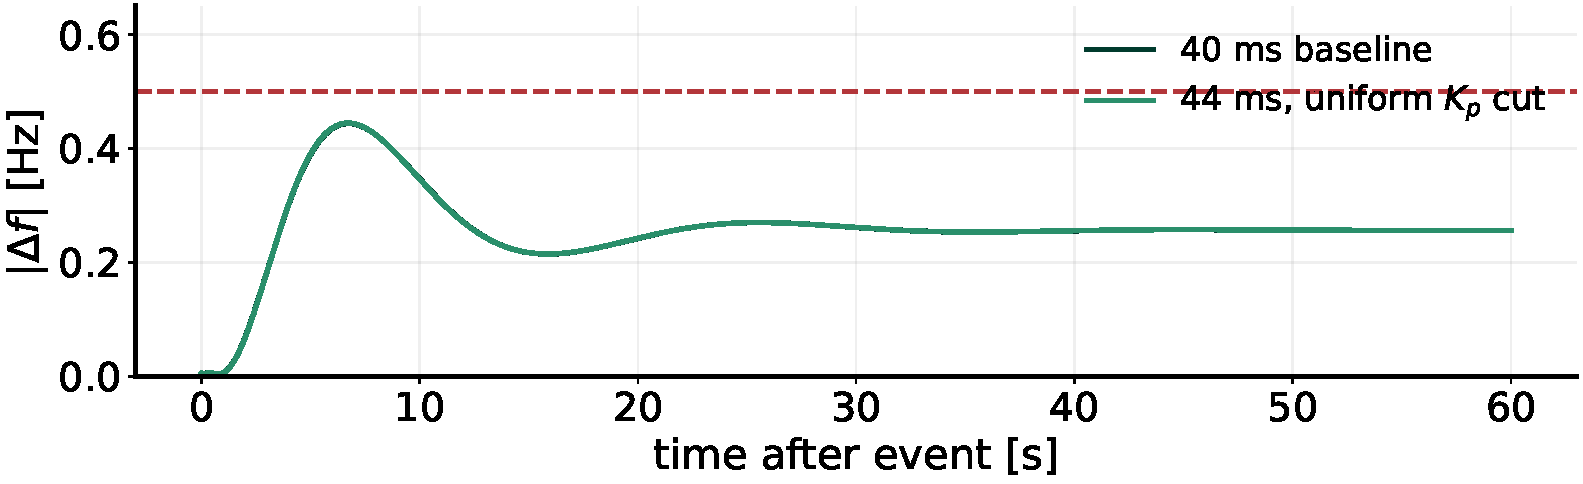
\includegraphics[width=268mm,height=82mm,keepaspectratio]{generated/figures/traj_events.pdf}\par
    {\fontsize{20pt}{23pt}\selectfont Load step $+100$ MW at bus 16: max bus-frequency deviation.\par}
    \vspace{0.5mm}
    {\fontsize{20pt}{23pt}\selectfont
    \begin{tabular}{@{}lccc@{}}
      \textbf{design} & \textbf{events} & \textbf{max $|\Delta f|$} & \textbf{slack}\\\hline
      baseline, 40 ms & 5/5 & 0.471 & 0.0074\\
      uniform $K_p$ $-14\,\%$, 44 ms & 5/5 & 0.472 & 0.0072\\
      6-site sparse, 44 ms & 4/5 & 0.492 & 0.0014\\
      no retune, 44 ms & abort & -- & --\\
    \end{tabular}\par}
    \vspace{0.5mm}
    {\fontsize{20pt}{23pt}\selectfont \textbf{Limits.} Floating-point counts, not certified; four-site retuning and the reduced-model 7--8 Hz family were refuted; five events are a finite campaign.\par}

    \vspace{2mm}
    \begin{tcolorbox}[colback=IASPaleGold,colframe=IASGold,boxrule=0.8pt,arc=1.5mm,left=2mm,right=2mm,top=1mm,bottom=1mm]
      {\fontsize{21pt}{25pt}\selectfont\textbf{TAKE-HOME} The closure is local (cycle 35--36, strongest couplings); the repair is global (one common $K_p$ cut). Sparse retuning of the core did not work in the full grid.\par}
    \end{tcolorbox}

  \end{PosterPanel}
\end{minipage}%
}%
\ifdefined\PosterFull
  \PosterSectionContent
  \let\PosterSectionFinish\relax
\else
  \def\PosterPageWidth{\PosterPreviewHalfPageWidth}
  \def\PosterPageHeight{\PosterPreviewLowerPageHeight}
  \def\PosterPreviewLeft{\PosterPreviewHalfLeft}
  \documentclass[final]{beamer}
% Fixed outer geometry for the IAS 2026 poster and its standalone previews.
% Edit this file only when changing the composition of the whole poster.
\def\PosterLayoutLoaded{1}
\newcommand{\PosterOuterMargin}{23mm}
\newcommand{\PosterColumnGap}{8mm}
\newcommand{\PosterRowGap}{4mm}
\newcommand{\PosterGridWidthMm}{868.4}
\newcommand{\PosterGridWidth}{\PosterGridWidthMm mm}
\newcommand{\PosterIdentityLeft}{8mm}
\newcommand{\PosterIdentityWidthMm}{898.4}
\newcommand{\PosterIdentityWidth}{\PosterIdentityWidthMm mm}
\newcommand{\PosterIdentityHeightMm}{54}
\newcommand{\PosterGreenHeightMm}{86}
\newcommand{\PosterHeaderHeightMm}{140}
\newcommand{\PosterHeaderHeight}{\PosterHeaderHeightMm mm}
\newcommand{\PosterGreenInset}{15mm}
\newcommand{\PosterHeaderTopOffset}{-3mm}
\newcommand{\PosterPhysicalPageWidthCm}{91.44}
\newcommand{\PosterPhysicalPageHeightCm}{106.68}

\newcommand{\PosterColWidth}{284.13mm}

\newcommand{\PosterRowHeight}{258mm}
\newcommand{\PosterRowHeightC}{352mm}
\newcommand{\PosterRowHeightA}{200mm}
% Module envelopes: width x height. Interior drawings remain local to each file.
\newcommand{\PosterOneWidth}{224mm}
\newcommand{\PosterTwoWidth}{412.4mm}
\newcommand{\PosterThreeWidth}{216mm}
\newcommand{\PosterTopRowHeight}{200mm}
\newcommand{\PosterStripHeight}{44mm}
\newcommand{\PosterFourHeight}{140mm}
\newcommand{\PosterHalfWidth}{430.2mm}
\newcommand{\PosterMiddleRowHeight}{140mm}
\newcommand{\PosterLowerRowHeight}{160mm}
\newcommand{\PosterBottomRowHeightMm}{84}
\newcommand{\PosterBottomRowHeight}{\PosterBottomRowHeightMm mm}

% Preview page sizes are centimetre numbers consumed by beamerposter.
\newcommand{\PosterPreviewTop}{6mm}
\newcommand{\PosterPreviewFullPageWidth}{\PosterPhysicalPageWidthCm}
\newcommand{\PosterPreviewWhitePageHeight}{8.0}
\newcommand{\PosterPreviewGreenPageHeight}{11.2}
\newcommand{\PosterPreviewTopRowPageHeight}{22.6}
\newcommand{\PosterPreviewStripPageHeight}{7.0}
\newcommand{\PosterPreviewFourPageHeight}{16.6}
\newcommand{\PosterPreviewMiddlePageHeight}{16.4}
\newcommand{\PosterPreviewLowerPageHeight}{18.6}
\newcommand{\PosterPreviewBottomPageHeight}{11.0}
\newcommand{\PosterPreviewOnePageWidth}{24.8}
\newcommand{\PosterPreviewTwoPageWidth}{43.6}
\newcommand{\PosterPreviewThreePageWidth}{23.84}
\newcommand{\PosterPreviewHalfPageWidth}{46.2}
\newcommand{\PosterPreviewOneLeft}{12mm}
\newcommand{\PosterPreviewTwoLeft}{11.8mm}
\newcommand{\PosterPreviewThreeLeft}{11.2mm}
\newcommand{\PosterPreviewHalfLeft}{15.9mm}

\usepackage[size=custom,width=\PosterPageWidth,height=\PosterPageHeight,scale=1.0]{beamerposter}
\usepackage{fontspec}
\usepackage{unicode-math}
\usepackage{amsmath,amssymb,mathtools}
\usepackage{graphicx}
\usepackage{tikz}
\usetikzlibrary{calc,positioning,shapes.geometric,shapes.misc,arrows.meta,patterns}
\usepackage{pgfplots}
\pgfplotsset{compat=1.18}
\usepackage{booktabs,tabularx,array}
\usepackage{ragged2e}
\usepackage[most]{tcolorbox}
\tcbuselibrary{skins,breakable}

% Shared visual roles and components, then scientific values used by the sections.
\input{poster_design_system.tex}
\input{generated/results.tex}
\input{generated/claims.tex}

\begin{document}

  \begin{frame}[t]
  \vspace*{\PosterPreviewTop}
  \noindent\hspace*{\PosterPreviewLeft}%
  \PosterSectionContent
  \end{frame}
  \def\PosterSectionFinish{\end{document}
}
\fi
\PosterSectionFinish
\par
\vspace{\PosterRowGap}
\noindent\hspace*{\PosterOuterMargin}%
% References, takeaway, contact, and QR
\long\def\PosterSectionContent{%
  \begin{tikzpicture}[x=1mm,y=1mm]
    \useasboundingbox (0,0) rectangle (\PosterGridWidthMm,\PosterBottomRowHeightMm);
    \fill[IASDeepGreen] (0,0) rectangle (\PosterGridWidthMm,\PosterBottomRowHeightMm);
    \fill[IASGold] (0,81) rectangle (\PosterGridWidthMm,\PosterBottomRowHeightMm);
    \fill[IASHeaderGreen] (350,0) rectangle (\PosterGridWidthMm,81);
    \fill[IASMidGreen] (700,0) rectangle (\PosterGridWidthMm,81);
    \fill[IASGold] (349,9) rectangle (350,72);
    \fill[IASGold] (699,9) rectangle (700,72);

    \node[anchor=north west,inner sep=0pt,font={\PosterFooterKickerType},text=IASGold] at (22,77) {TAKEAWAY};
    \node[anchor=north west,inner sep=0pt,font={\PosterFooterTitleType},text=IASWhite] at (22,68) {PRESERVING ONE MODE};
    \node[anchor=north west,inner sep=0pt,font={\PosterFooterTitleType},text=IASWhite] at (22,49) {DOES NOT PROTECT THE GRID.};
    \node[anchor=north west,inner sep=0pt,text width=312mm,align=left,font={\fontsize{25pt}{29pt}\selectfont},text=IASPaleGreen] at (22,29)
      {The gains that hide a delay from one mode are exact. The network decides what they do to all the others.};

    \node[anchor=north west,inner sep=0pt,font={\PosterFooterReferenceHeadingType},text=IASGold] at (364,77) {REFERENCES};
    \node[anchor=north west,inner sep=0pt,text width=166mm,align=left,font={\PosterFooterReferenceType},text=IASWhite] at (364,66)
      {[1] Markovi\'c et al., IEEE Trans. Power Syst., 2021.};
    \node[anchor=north west,inner sep=0pt,text width=166mm,align=left,font={\PosterFooterReferenceType},text=IASWhite] at (364,52)
      {[2] Huang et al., arXiv:1903.05489.};
    \node[anchor=north west,inner sep=0pt,text width=166mm,align=left,font={\PosterFooterReferenceType},text=IASWhite] at (364,38)
      {[3] Michiels \& Gumussoy, arXiv:2003.05496.};
    \node[anchor=north west,inner sep=0pt,text width=160mm,align=left,font={\PosterFooterReferenceType},text=IASWhite] at (534,66)
      {[4] D\"orfler et al., IEEE Trans. Power Syst., 2014.};
    \node[anchor=north west,inner sep=0pt,text width=160mm,align=left,font={\PosterFooterReferenceType},text=IASWhite] at (534,52)
      {[5] Bindel \& Hood, SIAM J. Matrix Anal. Appl., 2013.};
    \node[anchor=north west,inner sep=0pt,text width=160mm,align=left,font={\PosterFooterReferenceType},text=IASWhite] at (534,38)
      {[6] Johansson, IEEE Trans. Comput., 2017.};
    \node[anchor=north west,inner sep=0pt,text width=318mm,align=left,font={\PosterFooterReferenceType},text=IASPaleGreen] at (364,22)
      {Topics: [1] converter small-signal stability; [2] PLL stability and grid structure; [3] fixed-order design with delays; [4] sparse wide-area control; [5] nonlinear eigenvalues; [6] interval arithmetic.};

    \node[anchor=north west,inner sep=0pt,font={\PosterFooterContactHeadingType},text=IASGold] at (714,77) {CONTACT};
    \node[anchor=north west,inner sep=0pt,font={\PosterFooterContactNameType},text=IASWhite] at (714,66) {Jorge Luis Mayorga Taborda};
    \node[anchor=north west,inner sep=0pt,font={\PosterFooterContactLineType},text=IASPaleGreen] at (714,55) {jl.mayorga@uniandes.edu.co};
    \node[anchor=north west,inner sep=0pt,font={\PosterFooterContactLineType},text=IASPaleGreen] at (714,46) {Universidad de los Andes};
    \node[anchor=north west,inner sep=0pt,font={\PosterFooterContactLineType},text=IASPaleGreen] at (714,37) {Bogot\'a, Colombia};
    \node[anchor=north west,inner sep=0pt,font={\PosterFooterContactLineType},text=IASGold] at (714,24) {IEEE IAS Annual Meeting 2026};
    \node[anchor=north west,inner sep=0pt,font={\PosterFooterContactLineType},text=IASGold] at (714,15) {Vancouver, Canada};
  \end{tikzpicture}\par%
}%
\ifdefined\PosterFull
  \PosterSectionContent
  \let\PosterSectionFinish\relax
\else
  \def\PosterPageWidth{\PosterPreviewFullPageWidth}
  \def\PosterPageHeight{\PosterPreviewBottomPageHeight}
  \def\PosterPreviewLeft{\PosterOuterMargin}
  \documentclass[final]{beamer}
% Fixed outer geometry for the IAS 2026 poster and its standalone previews.
% Edit this file only when changing the composition of the whole poster.
\def\PosterLayoutLoaded{1}
\newcommand{\PosterOuterMargin}{23mm}
\newcommand{\PosterColumnGap}{8mm}
\newcommand{\PosterRowGap}{4mm}
\newcommand{\PosterGridWidthMm}{868.4}
\newcommand{\PosterGridWidth}{\PosterGridWidthMm mm}
\newcommand{\PosterIdentityLeft}{8mm}
\newcommand{\PosterIdentityWidthMm}{898.4}
\newcommand{\PosterIdentityWidth}{\PosterIdentityWidthMm mm}
\newcommand{\PosterIdentityHeightMm}{54}
\newcommand{\PosterGreenHeightMm}{86}
\newcommand{\PosterHeaderHeightMm}{140}
\newcommand{\PosterHeaderHeight}{\PosterHeaderHeightMm mm}
\newcommand{\PosterGreenInset}{15mm}
\newcommand{\PosterHeaderTopOffset}{-3mm}
\newcommand{\PosterPhysicalPageWidthCm}{91.44}
\newcommand{\PosterPhysicalPageHeightCm}{106.68}

\newcommand{\PosterColWidth}{284.13mm}

\newcommand{\PosterRowHeight}{258mm}
\newcommand{\PosterRowHeightC}{352mm}
\newcommand{\PosterRowHeightA}{200mm}
% Module envelopes: width x height. Interior drawings remain local to each file.
\newcommand{\PosterOneWidth}{224mm}
\newcommand{\PosterTwoWidth}{412.4mm}
\newcommand{\PosterThreeWidth}{216mm}
\newcommand{\PosterTopRowHeight}{200mm}
\newcommand{\PosterStripHeight}{44mm}
\newcommand{\PosterFourHeight}{140mm}
\newcommand{\PosterHalfWidth}{430.2mm}
\newcommand{\PosterMiddleRowHeight}{140mm}
\newcommand{\PosterLowerRowHeight}{160mm}
\newcommand{\PosterBottomRowHeightMm}{84}
\newcommand{\PosterBottomRowHeight}{\PosterBottomRowHeightMm mm}

% Preview page sizes are centimetre numbers consumed by beamerposter.
\newcommand{\PosterPreviewTop}{6mm}
\newcommand{\PosterPreviewFullPageWidth}{\PosterPhysicalPageWidthCm}
\newcommand{\PosterPreviewWhitePageHeight}{8.0}
\newcommand{\PosterPreviewGreenPageHeight}{11.2}
\newcommand{\PosterPreviewTopRowPageHeight}{22.6}
\newcommand{\PosterPreviewStripPageHeight}{7.0}
\newcommand{\PosterPreviewFourPageHeight}{16.6}
\newcommand{\PosterPreviewMiddlePageHeight}{16.4}
\newcommand{\PosterPreviewLowerPageHeight}{18.6}
\newcommand{\PosterPreviewBottomPageHeight}{11.0}
\newcommand{\PosterPreviewOnePageWidth}{24.8}
\newcommand{\PosterPreviewTwoPageWidth}{43.6}
\newcommand{\PosterPreviewThreePageWidth}{23.84}
\newcommand{\PosterPreviewHalfPageWidth}{46.2}
\newcommand{\PosterPreviewOneLeft}{12mm}
\newcommand{\PosterPreviewTwoLeft}{11.8mm}
\newcommand{\PosterPreviewThreeLeft}{11.2mm}
\newcommand{\PosterPreviewHalfLeft}{15.9mm}

\usepackage[size=custom,width=\PosterPageWidth,height=\PosterPageHeight,scale=1.0]{beamerposter}
\usepackage{fontspec}
\usepackage{unicode-math}
\usepackage{amsmath,amssymb,mathtools}
\usepackage{graphicx}
\usepackage{tikz}
\usetikzlibrary{calc,positioning,shapes.geometric,shapes.misc,arrows.meta,patterns}
\usepackage{pgfplots}
\pgfplotsset{compat=1.18}
\usepackage{booktabs,tabularx,array}
\usepackage{ragged2e}
\usepackage[most]{tcolorbox}
\tcbuselibrary{skins,breakable}

% Shared visual roles and components, then scientific values used by the sections.
\input{poster_design_system.tex}
\input{generated/results.tex}
\input{generated/claims.tex}

\begin{document}

  \begin{frame}[t]
  \vspace*{\PosterPreviewTop}
  \noindent\hspace*{\PosterPreviewLeft}%
  \PosterSectionContent
  \end{frame}
  \def\PosterSectionFinish{\end{document}
}
\fi
\PosterSectionFinish

\end{frame}
\end{document}
